\documentclass[11pt]{article}
\usepackage[margin=1in]{geometry}
\usepackage{amsmath,amssymb,amsthm,bm}
\usepackage{booktabs,tabularx,longtable}
\usepackage{graphicx}
\usepackage{enumitem}
\usepackage{natbib}
\usepackage[hidelinks]{hyperref}
\newtheorem{definition}{Definition}
\newtheorem{theorem}{Theorem}
\newtheorem{proposition}{Proposition}
\newtheorem{corollary}{Corollary}

\title{Conditional Assembly of Gravity, Matter, and Abelian Gauge Terminals\\
from One Ordered Tau Descent\\
\large Tau Core Foundation Paper VII-A}
\author{Jozsef Olcsak}
\date{Last revised: 26 August 2026}

\begin{document}
\maketitle

\begin{abstract}
We ask whether the previously constructed Tau gravity, temporal, quantum,
matter and Abelian gauge terminals can descend from one ordered physical
source ledger rather than from independently fitted sector models. On a
stabilized morphological body we construct one once-counted post-body
effective functional whose effect, metric, gauge and clock-character
derivatives generate probabilities, stress, current and formal clock
response. Diffeomorphism and $U(1)$ gauge invariance yield the conditional
Einstein--Maxwell--matter equations, Ward/Bianchi identities and their
standard weak-field leaf. A disjoint occupation ledger prevents duplicate
classical/quantum stress, while exact countermodels show that standard-limit
agreement does not establish common Tau provenance.

On an occupied two-mode restriction, ROOT one-particle coherence and
transverse-traceless stress arise from one preparation without an additional
cross-terminal gain. Differential recovery is reduced to a source-rank
problem: after de-duplication, the ROOT increment over the common P1 row space
is fixed by one source-owned mixed Gram. The paper therefore gives a
conditional common-source assembly and a precise non-identifiability boundary,
not a first-principles derivation of Einstein--Hilbert or Maxwell action shapes,
not quantized geometry and not unrestricted physical parent realization. The
rank-seven P3 packet and scalar-15/RG specialization are now owned by Technical
Papers VII-B and VII-C respectively.  The inherited signed rank-four
clock/body section likewise does not identify projective-state measure with
body four-volume; terminal assembly cannot supply the missing connector. We
also prove a general observer-access factorization theorem: equal complete
access kernels define one parent quotient and unique image transports, whose
terminal decomposition may be observer-dependent. This is information-level
mixing only. Contextual quantum structure cannot be fully identified with a
classical noncontextual gravity terminal by access change alone.
\end{abstract}

\begin{center}
\fbox{\begin{minipage}{0.92\linewidth}\small
\textbf{Inputs from earlier papers.} Paper I supplies body-first descent;
Paper II typed finite support; Paper III recovery-correctable record transport;
Paper IV the parent-realization boundary; Paper V observer time; Paper VI the
conditional quantum terminal. Paper V also supplies the common M4
metrological quotient: one measured dimension-bearing anchor selects an SI
representative while all dimensionless clock--ruler terminals remain fixed.
Technical Paper VII-B owns the later
pointed-exterior pair/top closure and its class-relative occupation theorem;
the present paper uses only its support consequence and does not re-prove it.

\textbf{Results owned here.} Morphology-conditioned joint-terminal assembly,
the finite occupation criterion, one effective source, the disjoint stress
ledger, Ward/Bianchi consistency, standard-form classification inside the
declared leaf, ROOT--TT common preparation, Abelian directional activation,
the exact de-duplicated source-rank obstruction, and the general
observer-dependent terminal-mixing theorem and no-go boundary.
\end{minipage}}
\end{center}

\begin{center}
\fbox{\begin{minipage}{0.92\linewidth}\small
\textbf{Claim boundary.} The Einstein--Hilbert and Maxwell action shapes are
inputs of the declared standard Lorentzian leaf and are not derived from the
narrow Tau parent. The results below are conditional assembly theorems. They
do not prove that the unrestricted physical base--seed law realizes or
occupies the common packet, quantize the metric, derive non-Abelian gauge
occupation or reproduce the Standard-Model spectrum.
They also do not construct a full projective/body measure connector or derive
absolute length, time or action units from equality of terminal ranks. The
inherited common M4 unit frame is defined only up to its positive metrological
orbit; this paper neither adds another terminal gain nor predicts the decimal
SI representative. Dimensionless gauge normalization remains a separate
source-Hessian/spectral question.
Temporal actuality is also an upstream enriched source clause, not an extra
stress--energy component generated by terminal assembly.  EOCC may order an
adopted occurrence--action completion, but the equations assembled here do
not select literal Parent traversal, and its proto-order current must not be
identified with dark matter, dark energy or a continuing 4D energy injection
without a separately derived terminal stress map.
\end{minipage}}
\end{center}

\section*{Notation and packet map}
\begin{center}\small
\begin{tabularx}{0.94\linewidth}{@{}p{0.19\linewidth}X@{}}
\toprule
Symbol or packet & Role\\
\midrule
$P1$ & Gravity--time--radiation/matter differential packet.\\
ROOT & Occupied two-mode quantum one-particle descriptor; its normalized shape
is $\rho_{\rm ROOT}$ and its occupation magnitude is retained separately.\\
TT & Transverse--traceless metric/stress readout paired with ROOT.\\
$P3$ & Rank-seven primitive algebra/recovery packet, imported only at the
handoff from Technical Paper VII-B.\\
$J_{\rm phys}^{\rm lin}$ & Parent-side physical incidence on the source-frozen
linear quotient.\\
$K_*$ & Positive source metric/Hessian on the true-null quotient.\\
\bottomrule
\end{tabularx}
\end{center}

\section{Question and reading order}

\paragraph{Inherited observer co-descent convention.}
The observer is not an external endpoint added to the joint terminal ledger.
The symbol $O$ first labels a body-side carrier candidate; regular local
rank-four descent, stable observer--source quantization and a nonzero
record/effect jointly make it operational and co-produce its accessible 4D
world.  The terminal maps assembled here act on that occupied common support.
They do not create an observer, a body or an independent channel layer.

The paper owns the conditional arrow
\[
M_\tau\longrightarrow\text{one post-body source ledger}
\longrightarrow\{g,A,\Phi,\rho_O,\text{formal clock response}\}.
\]
It does not use terminal residuals to select $M_\tau$ and does not construct
the body from a readout. The proof order is source ownership, variational
derivatives, standard-limit controls, ROOT--TT common preparation and finally
source-rank non-identifiability.

\tableofcontents
\clearpage

\section{Inherited-results ledger}

\begin{table}[ht]
\centering\small
\begin{tabularx}{\textwidth}{@{}p{0.20\textwidth}p{0.19\textwidth}Xp{0.18\textwidth}@{}}
\toprule
Result & Owner & Status and assumptions & Use here\\
\midrule
Body-first descent & Paper I & conditional physical MVP & generative order\\
Typed incidence & Paper II & finite source theorem & occupied domains\\
Record recovery & Paper III & exact/approximate conditional theorem & observer terminal\\
Parent-law realization & Paper IV & present reduct does not entail full packet & claim boundary\\
Temporal descent & Paper V & conditional clock/causal leaf & time and weak limit\\
Quantum terminal & Paper VI & conditional complex/effect/QFT packet & $\Gamma_q$ and $\rho_O$\\
Morphology-conditioned readouts & theory hub & common-source assembly for an
occupied complete signature & typed terminal projections\\
Operation-generated occupation & theory hub & cyclic--surjective/root-positive criterion
inside a fixed source representation & block nonvanishing\\
P1 assembly & theory hub & conditional metric/time/radiation ledger & $g$, null radiation, stress\\
P3 Abel handoff & theory hub & conditional $Z_F=p_*K_Y$ & Maxwell/current sector\\
Pointed P3 exterior seed & theory hub & conditional orthonormal 256-vector
root orbit; full-rank nontracial countermodel & representation boundary\\
Support--port P3 synthesis & theory hub & commuting support flag, two ordered
ports, independent unit and smooth decoder; finite audit & rank-seven
source reconstruction\\
Tau-local composition origin & theory hub; reproved here & exact inside the
component-local no-bridge/no-hidden-global-relation class & two-leg record
and effect tensor algebra\\
Component-local P3 joint occupation & owned here & exact inside one
once-counted enriched common law; narrow-reduct selection disproved & joint
LC1--LC4 and rank-seven status\\
Scalar-15/type-II completion & theory hub P4 branch & class-relative
base--seed reconstruction, common-scale ratio and exact functional RG law;
unrestricted branch occupation open & downstream particle-sector handoff\\
\bottomrule
\end{tabularx}
\caption{Dependency and ownership ledger. No inherited conditional result is
promoted to an unrestricted physical parent-law theorem.}
\label{tab:dependencyledger}
\end{table}

For logical self-containment, Appendix~\ref{app:dependencycertificate}
restates every imported premise actually used below.  The paper labels in
Table~\ref{tab:dependencyledger} are provenance locators, not hidden
hypotheses: the conditional
arguments can be checked from the restated premises without accepting an
unquoted result from a companion manuscript.  Several listed papers provide
architectural context only and are not logical dependencies of the main
theorems.

\section{Morphology-conditioned assembly and occupation}

The inherited terminals are not treated as independent information channels.
Let the stabilized body and observer support determine one finite physical
source representation $\mathcal E_{*,O}$.  No direct-sum decomposition of
this source is assumed.  Instead, for the typed role set
\begin{equation}
\mathcal P=\{T,G,R,M,Q,A\},
\qquad
\mathcal Y_{\rm role}:=\bigoplus_{a\in\mathcal P}\mathcal Y_a,
\label{eq:rolecodomain}
\end{equation}
let $R_a:\mathcal E_{*,O}\to\mathcal Y_a$ be terminal-role maps and
$R=(R_a)_a:\mathcal E_{*,O}\to\mathcal Y_{\rm role}$ their stacked map.
The direct sum is therefore a de-duplicated \emph{role codomain}, not a claim
that the source information separates.  Common source directions may affect
several $R_a$ simultaneously; their overlap is measured by the joint kernel
and stacked rank of the $R_a$.

Let $A_O$ be the body- and observer-conditioned access map and let
$Q_O^{(a)}$ be a stable observer-relative resolution map.  The operational
terminals are
\begin{equation}
Y_O^{(a)}=Q_O^{(a)}R_a A_O\Xi_*,
\label{eq:typedterminals}
\end{equation}
for one occupied source representative $\Xi_*$.  Equality under the specified
$Q_O^{(a)}$, rather than a non-transitive distance threshold, defines the
resolved readout classes.  Thus observer-relative quantization remains part
of the full descent and is not replaced by the continuous source geometry.

\begin{proposition}[Conditional morphology-conditioned representation]
\label{prop:moprassembly}
Assume a stabilized body, one occupied complete source representation
$\mathcal E_{*,O}$, a source-owned typed ledger map, and stable resolution
maps $Q_O^{(a)}$.  Then all terminals in Eq.~\eqref{eq:typedterminals} are
functorial restrictions of one source representative.  Their common-source
ownership and once-counting follow without terminal-specific gains.  Different
terminal names do not by themselves imply independent information.  This is
a representation theorem for an already occupied complete source ledger; it
does not establish uniqueness among all admissible source functionals.
\end{proposition}

\begin{proof}
Body stabilization fixes the domain of $A_O$.  The single map $A_O\Xi_*$ is
then mapped by the typed $R_a$ and resolved only afterwards by
$Q_O^{(a)}$.  Consequently every terminal factors through the same occupied
representative and the same access map.  Any additional terminal gain would
be an extra source datum, contrary to the assumed complete ledger.  The
conclusion is role-completeness of this construction, not uniqueness under
field redefinitions, improvement terms or alternative ultraviolet
completions.
\end{proof}

Define the immediate shared descriptor
\(\Xi_{OS}:=A_O\Xi_*\) on the occupied source domain.  The complete declared
terminal atlas is therefore the typed product
\begin{equation}
 \mathfrak R_{OS}
 =
 \left\langle Q_{OS}^{(a)}\circ R_a
 \right\rangle_{a\in\mathcal P}
 \circ\Xi_{OS}.
 \label{eq:paper-vii-unified-terminal-atlas}
\end{equation}
This is a product of unlike codomains, not a sum of observables with
incompatible units.  It includes pure roles and any hybrid map that jointly
retains two or more role legs before the final stable quantizer.

The Paper-I common-ancestor theorem makes the assembly falsifiable.  A
candidate terminal \(R_{\rm new}\) belongs to this atlas exactly when it is
constant on \(\Xi_{OS}\)-fibres; locally on a regular connected-fibre branch,
\begin{equation}
 \ker D\Xi_{OS}\subseteq\ker DR_{\rm new}.
 \label{eq:paper-vii-ancestor-kernel}
\end{equation}
The declared stack recovers the whole local ancestor quotient exactly when
\begin{equation}
 \ker D\Xi_{OS}
 =
 \ker
 \begin{bmatrix}
  D(Q^{(T)}R_T)\\
  D(Q^{(G)}R_G)\\
  D(Q^{(R)}R_R)\\
  D(Q^{(M)}R_M)\\
  D(Q^{(Q)}R_Q)\\
  D(Q^{(A)}R_A)
 \end{bmatrix}.
 \label{eq:paper-vii-ancestor-completeness}
\end{equation}
Strict inclusion means that the terminals share the ancestor but do not
reconstruct it; violation of Eq.~\eqref{eq:paper-vii-ancestor-kernel} is an
actual bypass.  Neither case may be repaired by fitting a terminal gain.
Physical no-bypass and completion of the terminal family remain upstream
source-occupation obligations.

Let $\mathfrak A_{\rm src}$ be the source-owned operation algebra and
$\Omega_s$ the occupied source vector, and define
$V_s:=\operatorname{span}(\mathfrak A_{\rm src}\Omega_s)$.

\begin{definition}[Activation and full occupation]
A required terminal role $a$ is \emph{activated} when $R_a(V_s)\neq\{0\}$.
It is \emph{fully occupied} when
\begin{equation}
R_a(V_s)=\mathcal Y_a.
\label{eq:fulloccupation}
\end{equation}
Full occupation implies activation; the converse need not hold.
\end{definition}

Assembly does not by itself prove either property.  In finite dimension, full
occupation of every required role is equivalent to
\begin{equation}
R_a\!\left(\operatorname{span}(\mathfrak A_{\rm src}\Omega_s)\right)=\mathcal Y_a
\quad\text{for every required }a.
\label{eq:cyclicoccupation}
\end{equation}

\begin{proposition}[Operation-generated occupation criterion]
\label{prop:occupation}
If $\Omega_s$ is cyclic for $\mathfrak A_{\rm src}$ on
$\mathcal E_{*,O}$ and each required $R_a$ is surjective, then
Eq.~\eqref{eq:cyclicoccupation} holds and every required role is fully
occupied.  More weakly, let $X_0\geq0$ be the occupied root covariance with
$\operatorname{supp}X_0\subseteq V_s$, and let the source-owned path maps
$L_e$ preserve the occupied subspace, $L_e(V_s)\subseteq V_s$.  Define
\begin{equation}
X_a:=\sum_{e\in\mathcal P_a}R_aL_eX_0L_e^\dagger R_a^\dagger\geq0.
\label{eq:positivepaths}
\end{equation}
If $R_aL_eX_0^{1/2}\neq0$ for at least one $e\in\mathcal P_a$, then role $a$
is activated, but full rank is not implied.
\end{proposition}

\begin{proof}
Cyclicity gives $V_s=\mathcal E_{*,O}$; surjectivity then gives
$R_a(V_s)=\mathcal Y_a$.  In the weaker case, every summand in
Eq.~\eqref{eq:positivepaths} is positive semidefinite and
\begin{equation}
\operatorname{Tr}X_a
=\sum_{e\in\mathcal P_a}\|R_aL_eX_0^{1/2}\|_{\rm HS}^2.
\end{equation}
One nonzero path therefore implies $X_a\neq0$.  Because
$\operatorname{Ran}(L_eX_0^{1/2})\subseteq V_s$, its nonzero image lies in
$R_a(V_s)$ and hence proves activation.  It does not establish
Eq.~\eqref{eq:fulloccupation}.
\end{proof}

Propositions~\ref{prop:moprassembly} and \ref{prop:occupation} move the open
problem upward.  Once the common representation and its source operation law
are occupied, separate terminal selection is unnecessary.  What remains
unproved is that $B_\tau^{\rm phys}+s_U$ selects this representation, makes
$\Omega_s$ cyclic with surjective required role maps (or realizes the rooted
positive alternative), and chooses
the observer access and resolution maps.  Algebraic generation, terminal
agreement and post-handoff record completeness do not prove that prior
physical realization and occupation.

\section{The ordered Paper-VII ledger}

Let $y$ denote body coordinates, and write $z=(g,A,\Phi)$ for the variational
post-body geometry, Abelian gauge and occupied classical matter fields.  The
quantum preparation is instead a fixed positive trace-one boundary datum
$\rho_{\rm in,O}\geq0$, $\operatorname{Tr}\rho_{\rm in,O}=1$ for the in-in
contour.  It is not an unconstrained stationary field.

\begin{definition}[Once-counted ordered ledger]
The Paper-VII ledger is
\begin{equation}
\mathfrak L_7=\left(
\mathcal A_{\rm pre}[y;B,s],\ y_*,\
\Gamma_7[g,A,\Phi\mid y_*;\rho_{\rm in,O}],\
\operatorname{Desc}_{O\leftarrow y_*},\ \mathcal U
\right),
\end{equation}
where $D_y\mathcal A_{\rm pre}(y_*)=0$, the physical body Hessian is positive,
and
\begin{equation}
\Gamma_7=\Gamma_{\rm grav}[g\mid y_*]
+\Gamma_{\rm EM}[A,g\mid y_*]
+\Gamma_{\rm occ}[\Phi,A,g\mid y_*]
+\Gamma_q[A,g\mid y_*;\rho_{\rm in,O}]+\Gamma_{\rm ct}[A,g].
\label{eq:jointfunctional}
\end{equation}
Each occupied mode and each counterterm appears in exactly one summand.
Observer restriction is evaluated after stationarity and is not varied back
against $y_*$.  The state $\rho_{\rm in,O}$ fixes the CTP preparation; the
Euler equations vary $g$, $A$ and $\Phi$, not $\rho_{\rm in,O}$.  The unit
packet $\mathcal U$ is shared by every summand.
\end{definition}

\section{One effective source on each stationary body fiber}

The symbol $\Gamma_7$ need not be postulated as five unrelated pieces.  Let
$\varphi$ collect the occupied quantum fields, and for each declared outcome
family let the dimensionless constant probe $\eta_a$ couple to a normalized
POVM-effect insertion satisfying
$E_a\geq0$ and $\sum_aE_a=I$ (hence $0\leq E_a\leq I$).  Let $\vartheta$
denote the occupied clock character.  The source convention is chosen so that
\begin{equation}
\Gamma_{\rm PC}[\eta]
=\Gamma_{\rm PC}[0]+\sum_a\eta_a\,\mathsf E_a[\varphi],
\qquad
\langle\mathsf E_a\rangle=\operatorname{Tr}(\rho_OE_a).
\label{eq:effectcoupling}
\end{equation}
On the already selected stationary body $y_*$ define the doubled
closed-time-path influence functional
\begin{align}
\mathcal I_{\rm CTP}
&:=\Gamma_{\rm PC}[y_*;g^+,A^+,\vartheta^+,\eta^+,\varphi^+]\notag\\
&\quad-\Gamma_{\rm PC}[y_*;g^-,A^-,\vartheta^-,\eta^-,\varphi^-],
\label{eq:ctpaction}\\
\exp\!\left(\frac{i}{\hbar}W_O[g^\pm,A^\pm,\vartheta^\pm,\eta^\pm
\mid y_*;\rho_{\rm in,O}]\right)
&=\int_{\rho_{\rm in,O}}\!\mathcal D\varphi^+\mathcal D\varphi^-\,
\exp\!\left(\frac{i}{\hbar}\mathcal I_{\rm CTP}\right).
\label{eq:ineffective}
\end{align}
The initial boundary condition joins the two branches through the fixed
preparation $\rho_{\rm in,O}$, and the path integral includes the standard
final branch identification.  The in-in contour is required for real causal expectation
values \citep{Schwinger1961,Keldysh1965}.  For every doubled source write
$X_c=(X^++X^-)/2$ and $X_\Delta=X^+-X^-$.  All derivatives below mean
$\delta/\delta X_\Delta$ followed by the physical limit
$X_\Delta=0$, $X_c=X$; differentiating an already identified common branch
would instead lose the response by CTP normalization.  The construction is a
terminal representation of an atemporal ordered functional fibration, not a
parent-time history.  CTP evolution and observer restriction produce the
normalized output state $\rho_O$ used in Eq.~\eqref{eq:effectcoupling}; neither
$\rho_{\rm in,O}$ nor $\rho_O$ is varied as a local Euler field.
Renormalization gives one $W_O^{\rm ren}$ whose physical-limit difference
derivatives define
\begin{align}
p_a&=\frac{\delta W_O^{\rm ren}}{\delta\eta_a}\bigg|_{\eta=0}
=\operatorname{Tr}(\rho_OE_a)\in[0,1],
&\langle T^q_{\mu\nu}\rangle_{\rm ren}
&=-\frac{2}{\sqrt{-g}}\frac{\delta W_O^{\rm ren}}{\delta g^{\mu\nu}},
\label{eq:sourceowners1}\\
\langle J_q^\mu\rangle_{\rm ren}
&=-\frac{1}{\sqrt{-g}}\frac{\delta W_O^{\rm ren}}{\delta A_\mu},
&\mathcal R_O^{\rm clock}&=\frac{\delta W_O^{\rm ren}}{\delta\vartheta}.
\label{eq:sourceowners2}
\end{align}
Consequently $\sum_a p_a=1$ within each normalized outcome family.  Without
the POVM and source-coupling conditions, the derivative would be only a
generic operator expectation and could not be identified as a Born
probability.
Here the effect-source renormalization convention is required to preserve the
POVM normalization at $\eta=0$; Eq.~\eqref{eq:effectcoupling} is an admitted
operational insertion and not a claim that every POVM has a local polynomial
field representation.
The final expression is schematic until the clock character and its
normalization are fixed, but its ownership is unambiguous.
The minus sign in the current definition is fixed by the Maxwell convention
$\Gamma_{\rm EM}=-(Z_F/4)\int\sqrt{-g}\,F^2$: stationarity then gives
$\nabla_\mu(Z_FF^{\mu\nu})=J^\nu$.  We use the same sign convention for the
classical current,
$J_{\rm cl}^\mu:=-(\sqrt{-g})^{-1}\delta\Gamma_{\rm occ}/\delta A_\mu$.

\begin{theorem}[Effective common-source construction]
\label{thm:effectivesource}
Assume the ordered pre-body solve, a source-owned probe-complete post-body
functional $\Gamma_{\rm PC}$, an observer-admissible integration class
$\mathcal C_O$ with fixed normalized boundary state
$\rho_{\rm in,O}$, and a local covariant, anomaly-free renormalization
prescription for the symmetries used below.  Then
Eqs.~\eqref{eq:ineffective}--\eqref{eq:sourceowners2}, together with the
classical body and coherent mean-field terms, construct the Paper-VII
$\Gamma_7$ ledger from one post-body source functional.  The construction is
complete at the level of the declared physical roles, modulo relocation of a
finite local counterterm between the geometric and quantum bookkeeping
columns while holding their sum fixed.  No uniqueness claim is made across
field redefinitions, improvement terms or inequivalent microscopic
functionals.
\end{theorem}
\begin{proof}
Functional differentiation of one $W_O^{\rm ren}$ gives the four displayed
terminal owners.  Diffeomorphism and gauge invariance give their common Ward
covector.  The fluctuation Green operator is the inverse of the corresponding
gauge-fixed Hessian on the physical quotient (or its prescribed generalized
inverse when zero modes remain) and therefore computes response; inserting it again as an
action summand would duplicate the fluctuation contribution.  A finite local
counterterm can be written in either the geometric or renormalized quantum
column, but linearity of variation shows that only the sum affects the field
equations.  Including the same term in both columns doubles its variation.
Thus this assumed functional supplies a consistent role ledger, while its
harmless counterterm placement convention is not fixed.  The argument does
not exclude a distinct probe-complete functional with the same terminal
equations.
\end{proof}

\paragraph{Scope.}
Theorem~\ref{thm:effectivesource} is a construction theorem inside the
selected ordered completion.  It does not show that the physical base--seed
law selects $\Gamma_{\rm PC}$, $\mathcal C_O$, its field spectrum or its
renormalized continuum measure.

The ordering is structural. If $H_B,H_P>0$ and the post-body equations have
body derivative $C$, the linear response is lower triangular:
\begin{equation}
\begin{pmatrix}\delta y\\\delta z\end{pmatrix}
=\begin{pmatrix}H_B^{-1}&0\\-H_P^{-1}CH_B^{-1}&H_P^{-1}\end{pmatrix}
\begin{pmatrix}\delta j_B\\\delta j_P\end{pmatrix}.
\label{eq:triangular}
\end{equation}
Thus morphology conditions the physical terminals, while a later terminal
load does not rebuild the body.

\begin{proposition}[Simultaneous-action no-go]
For an invertible positive simultaneous Hessian
\begin{equation}
\mathbb H=\begin{pmatrix}H_B&C^\dagger\\C&H_P\end{pmatrix},
\end{equation}
exact vanishing of body response to every pure post-body load implies $C=0$.
Hence nonzero body conditioning and exact body freeze cannot both be encoded
by one simultaneous unconstrained Hessian solve.
\end{proposition}
\begin{proof}
Schur inversion gives
$\delta y=-H_B^{-1}C^\dagger
(H_P-CH_B^{-1}C^\dagger)^{-1}\delta j_P$.
If this vanishes for every $\delta j_P$, invertibility forces $C=0$.
\end{proof}

\section{Disjoint occupation and stress ownership}

Let the occupied mode labels form a disjoint union
\begin{equation}
\mathcal I_{\rm occ}=\mathcal I_{\rm cl}\sqcup\mathcal I_q.
\label{eq:partition}
\end{equation}
Classical coherent modes represented in $\Gamma_{\rm occ}$ are excluded from
the state-dependent part of $\Gamma_q$; vacuum polarization and local
renormalization terms occur only in $\Gamma_q+\Gamma_{\rm ct}$.
This disjoint partition is a sufficient transparent ledger, not the only
possible field-theoretic organization. A background-field, one-particle-
irreducible or two-particle-irreducible construction is also admissible when
its mean field, fluctuation determinant and counterterms are derived from one
effective action and no full contribution is inserted twice.

\begin{proposition}[Duplicate-stress no-go]
If one nonzero occupied mode $i$ is included in both $\mathcal I_{\rm cl}$ and
$\mathcal I_q$ with the same metric variation, its stress contribution is
counted twice. No terminal redefinition removes this without changing the
metric equation or adding a compensating subtraction.
\end{proposition}
\begin{proof}
Metric variation is linear. The duplicated summands give
$-2(\sqrt{-g})^{-1}\delta(\Gamma_i+\Gamma_i)/\delta g^{\mu\nu}
=2T^{(i)}_{\mu\nu}$. A subtraction merely moves the ownership entry and must
therefore be recorded explicitly in $\Gamma_{\rm ct}$.
\end{proof}

\section{Joint terminal theorem}

The theorem below begins only after the upstream geometry gates have been
passed.  Gate G4a is existence of a Lorentz-conformal realization of the
source-owned cone/order on a regular smooth rank-four leaf; this is open in
the present Tau source.  Gate G4b is the standard conditional uniqueness of
the conformal class under the required distinguishing causality hypotheses.
A compatible source-owned density may then fix a representative only under
additional normalization assumptions.  Local coframes
$e_{(\alpha)}^A{}_{\mu}$ are related on overlaps by
$SO^+(1,3)$ transition functions and satisfy
\[
 g_{\mu\nu}|_{U_\alpha}
 =e_{(\alpha)}^A{}_{\mu}e_{(\alpha)}^B{}_{\nu}\eta_{AB}.
\]
Nothing in the conditional standard-leaf theorem asserts a single global
coframe, a spin lift, or the DA--ROOT/M4TR same-carrier intertwiner.  Those
remain separate topology and source-ownership obligations.

\begin{proposition}[Conditional standard-leaf form selector]
\label{prop:standardforms}
Assume that the selected readout leaf is a smooth four-dimensional Lorentzian
manifold.  Suppose the pure geometric action is local, diffeomorphism
invariant, metric-only, and has metric Euler equations of at most second
derivative order.  Suppose also that the Abelian action is local,
$U(1)$-gauge invariant, parity even, quadratic in first derivatives of $A$,
contains no derivatives of $F$, and has a constant positive kinetic
coefficient.  Then, up to boundary and four-dimensional topological terms,
the two actions have the forms
\begin{align}
\Gamma_{\rm grav}&=\frac{1}{2\kappa}\int d^4x\sqrt{-g}(R-2\Lambda),\\
\Gamma_{\rm EM}&=-\frac{Z_F}{4}\int d^4x\sqrt{-g}\,F_{\mu\nu}F^{\mu\nu},
\qquad Z_F>0.
\end{align}
The proposition fixes the action shapes inside this infrared class, but not
$\kappa$, $\Lambda$, $Z_F$, or physical realization of the class itself.
\end{proposition}
\begin{proof}
The four-dimensional Lovelock classification leaves only the cosmological and
Einstein tensors in the local metric-only second-order Euler tensor; the
Gauss--Bonnet density is topological in four dimensions
\citep{Lovelock1971}.  Integration gives the Einstein--Hilbert form up to
boundary/topological terms and overall normalization.  Abelian gauge
invariance restricts a local first-derivative action to dependence on
$F=dA$.  In four dimensions the quadratic Lorentz scalars are
$F_{\mu\nu}F^{\mu\nu}$ and
$F_{\mu\nu}\widetilde F^{\mu\nu}$.  Parity removes the second from the
dynamical class (and for constant coefficient it is topological), so the
first is unique up to $Z_F$; positivity fixes its sign.  These classification
arguments neither fix the coefficients nor prove that the parent selects
their hypotheses.
\end{proof}

The selector does not rule out higher-curvature gravity, torsion, additional
geometric fields, nonlinear electrodynamics or parity-odd sectors; those lie
outside its hypotheses.  Its content is uniqueness within the declared
standard infrared class, not uniqueness among all physical completions.

For the joint theorem adopt Proposition~\ref{prop:standardforms}, the
conditional common-source handoff $Z_F=p_*K_Y$, and a matter functional,
quantum measure and renormalization prescription that are diffeomorphism and
$U(1)$ gauge invariant and anomaly-free in those symmetries.  The handoff
removes an independent Maxwell gain inside the declared completion; it does
not evaluate $p_*$ or select the occupied representation trace $K_Y$ from the
physical parent.

\begin{theorem}[Common-descent Einstein--Maxwell--matter assembly]
\label{thm:assembly}
Under the ordered ledger, disjoint occupation rule, common unit packet and the
stated invariances, stationarity of Eq.~\eqref{eq:jointfunctional} with
$\rho_{\rm in,O}$ held fixed gives
\begin{align}
G_{\mu\nu}+\Lambda g_{\mu\nu}
&=\kappa\left(T^{\rm EM}_{\mu\nu}+T^{\rm cl}_{\mu\nu}
+\langle T^q_{\mu\nu}\rangle_{\rm ren}\right),
\label{eq:einstein}\\
\nabla_\mu(Z_FF^{\mu\nu})
&=J_{\rm cl}^{\nu}+\langle J_q^\nu\rangle_{\rm ren}.
\label{eq:maxwell}
\end{align}
On the matter and gauge equations, the Ward identities and Bianchi identity
imply
\begin{equation}
\nabla^\mu T^{\rm tot}_{\mu\nu}=0,
\qquad
\nabla_\mu J_{\rm tot}^{\mu}=0.
\label{eq:ward}
\end{equation}
No additional gravity, gauge or quantum-backreaction gain is introduced at the
terminal stage.
\end{theorem}
\begin{proof}
Equations \eqref{eq:einstein} and \eqref{eq:maxwell} are the metric and gauge
Euler equations of the single post-body functional. Gauge invariance gives
current conservation. Diffeomorphism invariance gives the combined stress
Ward identity, including the Lorentz-force exchange between matter and gauge
sectors. The divergence of the left side of Eq.~\eqref{eq:einstein} vanishes
identically, so the equations are mutually consistent. Disjoint occupation
and the single-entry counterterm ledger ensure that each contribution is varied
once.
\end{proof}

\begin{corollary}[Standard weak-field leaf]
For $g_{00}=-(1+2\Phi_N/c^2)$, stationary weak fields, nonrelativistic
sources and a local patch whose boundary data admit the Newtonian limit,
Eq.~\eqref{eq:einstein} reduces to
\begin{equation}
\nabla^2\Phi_N=4\pi G\rho_{\rm tot}-\Lambda c^2,
\end{equation}
where $\rho_{\rm tot}$ is the same once-counted density appearing in the
ledger.  On scales $L\ll |\Lambda|^{-1/2}$, or for $\Lambda=0$, the final term
is negligible and the ordinary Poisson equation follows. Equation
\eqref{eq:maxwell} reduces to the ordinary Maxwell equations after the
inherited field normalization. This is standard recovery, not a Tau-specific
deviation.
\end{corollary}

\section{Relation to established frameworks}

The use of one renormalized effective action and its metric variation belongs
to semiclassical gravity and curved-spacetime QFT, not uniquely to Tau Core
\citep{Wald1977,BirrellDavies1982,HollandsWald2001}.  The closed-time-path
extension and stress-noise cumulants likewise parallel stochastic gravity
\citep{HuVerdaguer2008}.  Observer-relative descriptions have independent
precedent in quantum-reference-frame constructions
\citep{GiacominiCastroRuizBrukner2019}, while deriving Einstein dynamics from
more primitive thermodynamic data is exemplified by emergent-gravity programs
\citep{Jacobson1995}.

The finite-dimensional algebraic ingredients are also established
mathematics rather than Tau-specific discoveries.  The exterior realization
of Clifford multiplication is standard spin geometry
\citep{LawsonMichelsohn1989}; cyclic representations and their unitary
uniqueness belong to the GNS/operator-algebra framework
\citep{BratteliRobinson1979}; and special dagger--Frobenius structures provide
the finite-dimensional algebraic language for normalized copy/record data
\citep{Vicary2011,CoeckePavlovicVicary2013}.  Paper VII's claim is therefore
not novelty of these ingredients separately, but their conditional placement
in one source-owned, once-counted terminal ledger and the accompanying
non-identifiability controls.

Paper VII's narrower Tau-specific contribution is the body-first ordering,
the typed morphology-conditioned access and resolution maps, the explicit
once-counted cross-terminal ownership ledger, and the finite no-go separating
terminal agreement from common provenance.  The standard effective-action
machinery is used as a consistency leaf; it is not presented as evidence for
the Tau parent ontology.

\section{Local constraint structure}

The covariant equations must reproduce constraints, not only evolution
equations. Let $n^\mu$ be the unit normal to an observer-compatible spacelike
leaf, $h_{\mu\nu}=g_{\mu\nu}+n_\mu n_\nu$ its induced metric, and $K_{ij}$ its
extrinsic curvature. With
$\rho=n^\mu n^\nu T^{\rm tot}_{\mu\nu}$ and
$j_i=-h_i{}^\mu n^\nu T^{\rm tot}_{\mu\nu}$, the normal projections of
Eq.~\eqref{eq:einstein} give, in the stated sign convention,
\begin{align}
{}^{(3)}R+K^2-K_{ij}K^{ij}&=2\kappa\rho+2\Lambda,
\label{eq:hamconstraint}\\
D_j(K^{ij}-h^{ij}K)&=\kappa j^i.
\label{eq:momconstraint}
\end{align}
The normal projection of Eq.~\eqref{eq:maxwell} gives the Abelian Gauss
constraint
\begin{equation}
D_i(Z_FE^i)=\rho_J.
\label{eq:gaussconstraint}
\end{equation}
The Ward identities propagate these constraints when the classical and
quantum matter equations hold. Paper VII therefore imports the standard local
constraint architecture from the one joint functional; it does not derive a
new constraint algebra or quantize it.

\section{Primitive terminal inventory}

The assembled packet contains several typed outputs, not several names for
the same information:
\begin{center}
\small
\begin{tabularx}{0.96\textwidth}{@{}p{0.20\textwidth}Xp{0.25\textwidth}@{}}
\toprule
Family & Primitive terminal content & Derived or composite descendants\\
\midrule
Geometry/gravity & $g$, connection, curvature and constraints & proper time,
tidal response, lensing after a null source\\
Gauge/radiation & $A$, $F$, conserved current, two screen polarizations &
photon propagation, redshift and optical transport\\
Matter occupation & occupied localized or propagating solutions $\Phi$ &
mass, energy, stress and charge records\\
Quantum operation & $\rho$, effects, instruments and correctable composition &
Born statistics and renormalized quantum stress/current\\
Observer access & causal orientation, clock and stable restriction &
observer-relative terminal classes\\
\bottomrule
\end{tabularx}
\end{center}
Stress-energy, current, redshift and lensing are variational or composite
outputs of these families; they are not silently counted as new primitive
source directions. Conversely, the symmetric local gravity descriptor cannot
stand in for internal gauge charge, quantum phase or occupied matter. A global
information-completeness claim must wait for the non-Abelian and fermionic
known-terminal completions.

\section{Why the standard limit does not prove common provenance}

\begin{proposition}[Equal-terminal provenance no-go]
The equations \eqref{eq:einstein}--\eqref{eq:ward} do not imply that their
coefficients or sectors arise from one Tau source.
\end{proposition}
\begin{proof}
Construct two source models with the identical numerical effective functional
$\Gamma_7[g,A,\Phi]$.  In $C_{\rm joint}$ its sector coefficients are images
of one common source line and unit map.  In $C_{\rm sep}$ take four independent
source lines and choose their terminal coefficient maps to have the same
numerical images as the four coefficients in $C_{\rm joint}$.  The two models
therefore have identical functionals as functions of the terminal fields, so
all Euler equations, Ward identities and solution sets coincide.  Their
source ownership graphs are nevertheless non-isomorphic: one has a common
source line and the other has four independent lines.  Hence no observation
or algebraic manipulation of Eqs.~\eqref{eq:einstein}--\eqref{eq:ward} alone
can recover common provenance.  This is an identifiability counterexample,
not a claim that the independently sourced model is physically preferred.
\end{proof}

This no-go fixes the empirical interpretation: terminal data may test a
source-frozen forward ledger, but may not choose its source partition,
susceptibilities or unit map.

\begin{proposition}[Same-reduct selection no-go]
\label{prop:samereduct}
The currently frozen stationary body, common action line, observer quotient
and terminal type signatures do not entail physical occupation of the full
effective-source packet of Theorem~\ref{thm:effectivesource}.
\end{proposition}
\begin{proof}
Hold fixed the body $y_*$, its Hessian, common units, causal orientation and
observer quotient.  Add the same typed internal edge carrier
$\mathcal H_e=\mathbb C^2$ to both completions, with effect
\begin{equation}
E_e=\begin{pmatrix}0&0\\0&1\end{pmatrix},\qquad
\rho_w=\begin{pmatrix}1-w&0\\0&w\end{pmatrix},
\quad 0<w<1,\qquad c_0=0,\quad c_1=1.
\label{eq:counterpair}
\end{equation}
$\rho_w$ is positive, has unit trace and is invariant under the diagonal
$U(1)$ action.  A concrete covariant edge functional is supplied by
a charged scalar doublet $\chi\in\mathbb C^2$ with
\begin{equation}
\Gamma_e[\chi,g,A]
=-\int d^4x\sqrt{-g}\left[
g^{\mu\nu}(D_\mu\chi)^\dagger D_\nu\chi
+m_e^2\chi^\dagger\chi\right],
\qquad D_\mu=\partial_\mu-iqA_\mu I_2 .
\label{eq:counteredgeaction}
\end{equation}
It is diffeomorphism invariant, diagonal-$U(1)$ gauge invariant and has the
same positive internal state normalization in both completions.  Define
\begin{equation}
\Gamma_{\rm PC}^{(j)}[\eta_e]
=\Gamma_{\rm common}+\Gamma_e+c_j\eta_e\mathsf E_e,
\qquad j\in\{0,1\}.
\label{eq:counterprobes}
\end{equation}
At the physical source value $\eta_e=0$, both completions have exactly the
same action, state, body, Hessian, observer quotient, typed carrier,
covariance and normalization.  The frozen upstream reduct does not include a
law selecting the probe coefficient $c_j$.  Nevertheless,
\begin{equation}
\frac{\delta W_O^{(0)}}{\delta\eta_{e,\Delta}}\bigg|_{\rm phys}=0,
\qquad
\frac{\delta W_O^{(1)}}{\delta\eta_{e,\Delta}}\bigg|_{\rm phys}
=\operatorname{Tr}(\rho_wE_e)=w>0.
\end{equation}
Only $C_1$ contains the declared nonzero effect-source owner.  Since the full
effective-source packet includes that owner, the frozen upstream reduct does
not entail the complete packet.  The result concerns source ownership, not
the logically different statement that a realized POVM outcome must have
nonzero probability in every state.  No stress- or current-difference is
claimed because the physical unprobed action and field state are identical.
Additional source-owned occupation or an empirically discriminating
source-frozen prediction is required.
\end{proof}

This finite counterpair is the stopping result for the origin question at the
present source level.  It forbids both an unrestricted parent-law promotion of
Theorem~\ref{thm:effectivesource} and another same-level search for a hidden
normalization.  It does not weaken the conditional forward construction.

Figure~\ref{fig:jointledger} summarizes the resulting generative and
variational order.

\begin{figure}[t]
\centering
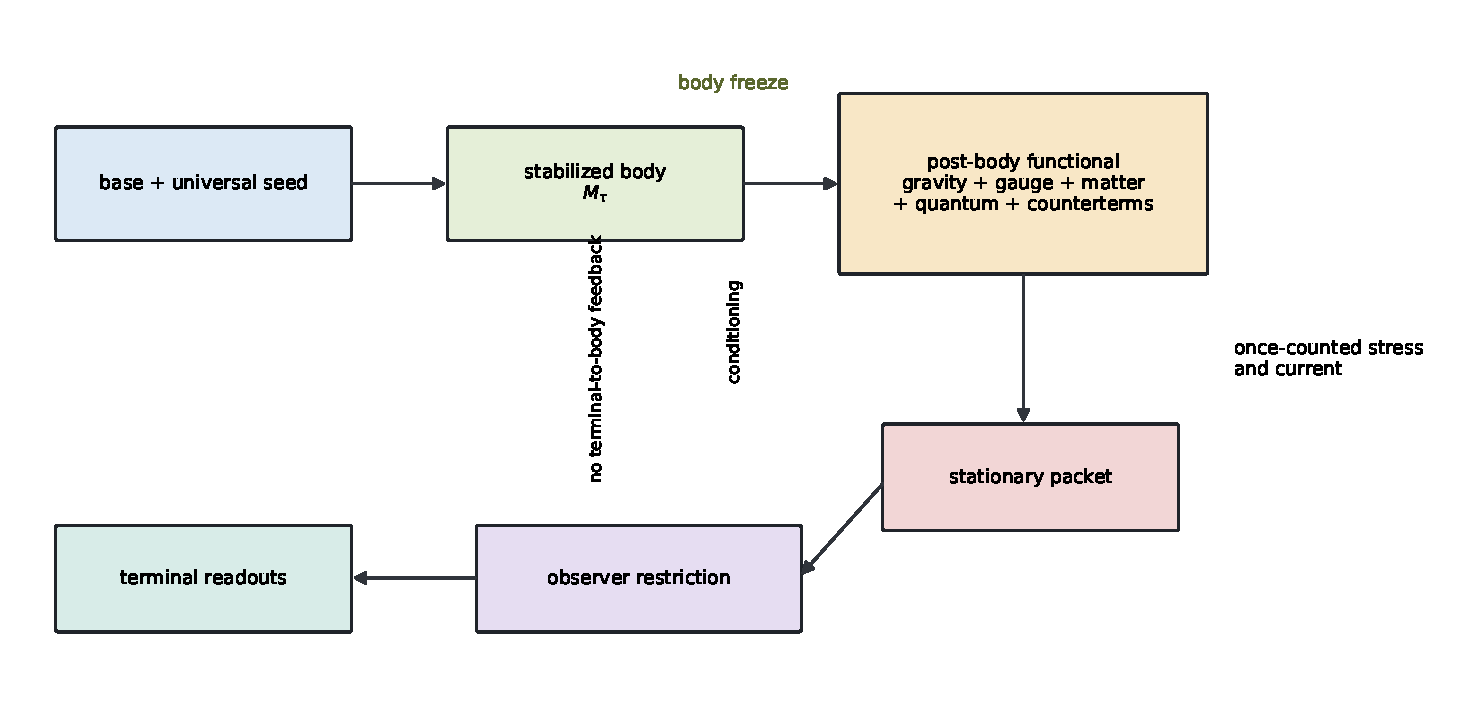
\includegraphics[width=0.92\textwidth]{figures/fig_joint_ledger.pdf}
\caption{Ordered common-source construction. The body is stabilized before the
post-body functional is solved; observer restriction is terminal.}
\label{fig:jointledger}
\end{figure}

\section{Quantum backreaction and the quantum-gravity boundary}

The quantum term in Eq.~\eqref{eq:einstein} is a renormalized expectation
value on a classical body-derived metric, in the standard semiclassical sense
\citep{BirrellDavies1982,Wald1977}. Local covariance and admissible
renormalization follow the usual curved-spacetime QFT framework
\citep{HollandsWald2001,BrunettiFredenhagenVerch2003}. The metric can also be
driven by a stress-noise second cumulant in a stochastic extension, but this
does not quantize geometry.

Paper VII therefore establishes a conditional quantum--gravity
\emph{interface}, not quantum gravity. A path integral or operator algebra for
the metric, gravitational gauge fixing, a physical inner product and a
nonperturbative ultraviolet completion remain absent.

\subsection{Observer-dependent terminal mixing and its exact boundary}

The common parent descriptor permits a sharper statement than either terminal
identity or terminal independence. Let $X$ be a fixed source-owned parent
tangent and let
\begin{equation}
 A_i:=\begin{pmatrix}Q_i\\G_i\end{pmatrix}:X\longrightarrow
 Y_{Q,i}\oplus Y_{G,i}
 \label{eq:jointobserveraccess}
\end{equation}
be the complete linearized quantum--gravity access of observer $O_i$, after
its stable quantizer, null quotient and calibration have been included.

\begin{proposition}[Joint-access mixing]
\label{prop:jointaccessmixing}
Two observers resolve the same parent quotient if and only if
\begin{equation}
 \ker A_1=\ker A_2.
 \label{eq:equalaccesskernels}
\end{equation}
In that case there is a unique isomorphism on the realized images,
$U_{21}:A_1(X)\to A_2(X)$, such that
\begin{equation}
 A_2=U_{21}A_1.
 \label{eq:accessfactorization}
\end{equation}
For any three equal-access observers these image transports satisfy
$U_{ki}=U_{kj}U_{ji}$, $U_{ii}=I$ and $U_{ij}=U_{ji}^{-1}$.
\end{proposition}

\begin{proof}
If Eq.~\eqref{eq:accessfactorization} holds with $U_{21}$ invertible, the two
kernels are equal. Conversely, define $U_{21}(A_1x):=A_2x$. Equality of the
kernels makes this independent of the representative $x$, and the same
construction with the indices exchanged gives its inverse. Uniqueness on
$A_1(X)$ is immediate. The groupoid identities follow by uniqueness of the
factorizations of $A_k$ through $A_i$.
\end{proof}

This permits observer-dependent terminal assignment without creating new
parent information. On a realized pure quantum sector
$E_{Q,1}:=A_1(X)\cap(Y_{Q,1}\oplus0)$, the intrinsic quantum-to-gravity
component is $\pi_{G,2}U_{21}|_{E_{Q,1}}$. An arbitrary extension of $U_{21}$
to the ambient direct sum is not unique when $A_1(X)$ is a proper subspace, so
its displayed off-diagonal matrix entries are not physical invariants. The
rank-two pure-swap witness
\begin{equation}
 Q_1=(1\;0),\quad G_1=(0\;1),\qquad
 Q_2=(0\;1),\quad G_2=(1\;0)
 \label{eq:pureswapwitness}
\end{equation}
proves mathematical nonemptiness only.

For unequal full kernels $K_i:=\ker A_i$, the maximal common linear quotient
and the combined quotient are respectively $X/(K_i+K_j)$ and
$X/(K_i\cap K_j)$. Their dimensions are
\begin{align}
 d_{\rm shared}^{ij}
 &=\operatorname{rank} A_i+\operatorname{rank} A_j
   -\operatorname{rank}\!\begin{pmatrix}A_i\\A_j\end{pmatrix},
 \label{eq:shareddimension}\\
 d_{\rm union}^{ij}
 &=\operatorname{rank}\!\begin{pmatrix}A_i\\A_j\end{pmatrix}.
 \label{eq:uniondimension}
\end{align}
These counts are invariant under invertible observer recalibration and must
be evaluated before named terminals are counted as independent.

Information equivalence is not physical sector duality. If a full role
exchange is represented by an injective multiplicative intertwiner $\Phi$,
then $\Phi([B,C])=[\Phi(B),\Phi(C)]$. Consequently a genuinely
noncommutative quantum operational algebra cannot be fully equivalent in this
sense to a commutative classical-gravity algebra. Morita equivalence alone is
too weak because it need not preserve element commutators or operational
probabilities. More generally, a full and faithful process equivalence that
preserves every closed-circuit probability would pull any classical
noncontextual simplex model of the gravity fragment back to the quantum
fragment. It therefore cannot connect a certified contextual quantum packet
to a gravity packet that remains classical under the same independently
frozen causal, dimension and memory assumptions.

Raw order dependence is not the required witness: classical transformations,
nonlinear backreaction, apparatus memory and unequal preparations can also
make $A\circ B$ differ from $B\circ A$. A finite physical promotion requires,
in order, (i) common-parent kernel reconstruction, (ii) independent
preparation/transformation/measurement equivalences, (iii) rejection of a
bounded commutative comparator by contextuality, incompatibility or equivalent
tomography, and (iv) one source-frozen map transporting both information and
composition. An unrestricted classical hidden-state automaton can encode any
finite behavior table, so the comparator bounds are indispensable.

The result generalizes to any typed terminal family
$A_i=\bigoplus_{\alpha}T_i^\alpha$. Equal full kernels give the same image
groupoid; pure $\alpha\to\beta$ exchange is tested on the carrier where all
competing terminal blocks vanish. Globally, Jacobian kernels must be replaced
by equality of the stable quantized fibers. This establishes a conditional
architecture in which the joint accessible parent quotient can be
observer-invariant while its terminal decomposition is observer-dependent.
It does not prove that Nature realizes nonzero cross-terminal mixing, that the
metric is quantized, or that quantum and gravity are ontologically identical.

The time block has no privileged information status inside this theorem. If
$T_O$ is the clock component of the complete stack $A_O$, every other
terminal factors through it exactly when $\ker T_O=\ker A_O$ locally, or when
their stable fibers coincide globally. A scalar rank-one clock therefore
cannot determine this paper's higher-rank joint terminal packet. The richer
ordered distinguishability carrier may constrain every terminal, but it is
upstream of and strictly differently typed from the clock projection.

\subsection{Post-body source origin of the access maps}

The preceding access maps need not be inserted independently. After body
stabilization, let $x\in X$ perturb the frozen parent descriptor and let
$z_i\in Z_i$ be the observer--source response. The positive post-body
quadratic germ
\begin{equation}
 \Phi_i^{(2)}(z_i;x)
 =\frac12\langle z_i,H_i z_i\rangle-\langle z_i,C_i x\rangle,
 \qquad H_i>0,
 \label{eq:accesssourcegerm}
\end{equation}
has stationary solution $z_i=H_i^{-1}C_i x$. If $L_i$ is the de-duplicated
resolved terminal exit, then
\begin{equation}
 \boxed{A_i=L_iH_i^{-1}C_i.}
 \label{eq:sourceaccessmap}
\end{equation}
Here $C_i$ is the parent/access mixed Hessian of the one post-body source law;
Eq.~\eqref{eq:sourceaccessmap} introduces no separate terminal capacity gain
and does not place the frozen body derivative back into a simultaneous solve.

The exact access fiber is
\begin{equation}
 \ker A_i=C_i^{-1}\!\left(H_i\ker L_i\right).
 \label{eq:sourceaccesskernel}
\end{equation}
Thus equal observer access requires equality of these preimages. If $L_i$ is
injective on the stationary response image, this reduces to
$\ker C_i=\ker C_j$; observer stiffness changes sensitivity but not the
accessible parent directions. For a lossy exit the full
Eq.~\eqref{eq:sourceaccesskernel} is required, and changing $H_i$ can rotate a
response into or out of the terminal null.

One common positive relation Hessian does not force equal access. Even when
\begin{equation}
 H_i=J_i^*K_RJ_i,
 \qquad C_i=J_i^*K_RJ_X,
 \label{eq:commonrelationhessian}
\end{equation}
different observer embeddings $J_i$ can select different coordinate
subspaces and hence different kernels. This gives an exact same-source
countermodel to the claim that common provenance itself implies terminal
mixing.

A sufficient source-selected route is a covariant observer orbit. If
\begin{equation}
 C_j=V_{ji}^{-*}C_i,\qquad
 H_j=V_{ji}^{-*}H_iV_{ji}^{-1},\qquad
 L_jV_{ji}=W_{ji}L_i,
 \label{eq:covariantaccessorbit}
\end{equation}
with invertible maps on the realized images, substitution into
Eq.~\eqref{eq:sourceaccessmap} gives
\begin{equation}
 A_j=W_{ji}A_i.
 \label{eq:sourceownedtransport}
\end{equation}
The observer transport is then derived from the source packet rather than
chosen after terminal inspection. Equation~\eqref{eq:covariantaccessorbit} is
a sufficient enriched-source condition, not a theorem that physical observers
occupy one such orbit. Off-diagonal physical terminal content of $W_{ji}$
remains unselected.

\subsection{Representation-overlap selection rule}

The covariant orbit law also restricts which off-diagonal blocks can exist.
If a physical symmetry group $\mathcal G$ acts on realized terminal sectors,
source covariance requires every cross-terminal component to lie in
\begin{equation}
 W_{ji}^{\beta\leftarrow\alpha}
 \in\operatorname{Hom}_{\mathcal G}(E_i^\alpha,E_j^\beta).
 \label{eq:terminalintertwiner}
\end{equation}
Schur's lemma therefore sets the component to zero between inequivalent
irreducible sectors. For compact $\mathcal G$, after complexification when
needed, write
\begin{equation}
 E_i^\alpha\simeq\bigoplus_\lambda
 M_{i,\alpha,\lambda}\otimes V_\lambda.
\end{equation}
Every covariant cross map is blockwise
$w_{ji,\lambda}^{\beta\leftarrow\alpha}\otimes I_{V_\lambda}$ and obeys
\begin{equation}
 \operatorname{rank} W_{ji}^{\beta\leftarrow\alpha}
 \leq\sum_\lambda
 \min\{\dim M_{i,\alpha,\lambda},\dim M_{j,\beta,\lambda}\}
 \dim V_\lambda.
 \label{eq:representationrankbound}
\end{equation}
Representation overlap is necessary, not sufficient: source normalization,
orientation, gauge descent and operational-law transport remain required.

This rule makes the ROOT--TT packet below the first current eligible
quantum--gravity pair. Its two-mode coherence and TT stress carry the same
oriented spin-two screen type. A scalar probability or spin-one current cannot
mix covariantly into that pure spin-two terminal without an additional
symmetry-breaking carrier. The ROOT--TT identity still proves only
common-preparation transport into semiclassical stress, not invertible
quantum--gravity role duality.

\subsection{Coupling is weaker than an intrinsically hybrid terminal}

For a positive joint quadratic packet
\begin{equation}
 K_{QG}=\begin{pmatrix}A&C\\C^*&B\end{pmatrix},
 \qquad A>0,\quad B>0,
 \label{eq:hybridpacket}
\end{equation}
$C\neq0$ proves coupling in the declared quantum/gravity splitting. It does
not prove absolute hybridity: an unrestricted triangular congruence produces
$A\oplus(B-C^*A^{-1}C)$. A meaningful hybrid claim must therefore freeze the
admissible transformations from terminal type, gauge, units, quantizer and
operational composition before inspecting $C$.

Under invertible block-preserving transformations,
$C\mapsto S_Q^*CS_G$ and $\operatorname{rank} C$ is invariant. Under independent
metric-preserving terminal frames, the singular values of
\begin{equation}
 M=A^{-1/2}CB^{-1/2}
 \label{eq:hybridspectrum}
\end{equation}
are invariant and satisfy $0\le\sigma_k(M)<1$ by positivity. Their nonzero
ordered set is a dimensionless typed quadratic-hybrid spectrum. It measures
normalized coupling, not physical quantum--gravity unification.

Physical hybridity additionally requires one occupied once-counted mixed
source block, survival through gauge/null/quantizer descent, resolved process
nonfactorization against a frozen typed comparator and preservation of both
operational signatures. The current ROOT--TT map passes representation
eligibility and common preparation but does not yet supply this occupied joint
Hessian or the operational nonfactorization theorem. It is therefore a
coupled candidate, not an established hybrid terminal.

The exact deterministic identity is in fact more restrictive.  Write its
retained linear form as $t=Kq$ and let $Sigma_Q>0$ be the ROOT covariance or
static susceptibility on its support.  Then
\begin{equation}
 \Gamma_{QT}=
 \begin{pmatrix}\Sigma_Q&\Sigma_QK^*\\
 K\Sigma_Q&K\Sigma_QK^*\end{pmatrix}
 =\begin{pmatrix}I\\K\end{pmatrix}\Sigma_Q
 \begin{pmatrix}I&K^*\end{pmatrix}.
 \label{eq:rootttgraphcovariance}
\end{equation}
Consequently $\operatorname{rank}\Gamma_{QT}=\operatorname{rank}\Sigma_Q$
and the TT-given-ROOT Schur residual vanishes.  Every nonzero canonical
correlation is unity on the supported image.  Thus the presently proved
ROOT--TT relation is a redundant graph of one shared preparation, lying on
the semidefinite boundary of the strictly positive family
in Eq.~\eqref{eq:hybridpacket}; it is not itself a two-sector hybrid proof.

The minimal covariance extension $t=Kq+\eta$ with
$\langle\eta q^*\rangle=0$ and $N:=\langle\eta\eta^*\rangle>0$ has Schur
residual exactly $N$ and is strictly positive.  This does not close the
physical argument: $N$ is a new underived TT source/noise and the same packet
has a classical Gaussian realization.  A nonarbitrary continuation must
instead reconstruct the connected mixed susceptibility of one renormalized
source functional,
\begin{equation}
 C_{QT}=\left.
 \frac{\delta^2 W[h_{TT},\eta_Q]}
 {\delta h_{TT}\,\delta\eta_Q}\right|_{0},
 \label{eq:rootttmixedsource}
\end{equation}
with contact and subtraction terms frozen, and must then prove quotient
survival and operational nonfactorization.  Equation~\eqref{eq:rootttidentity}
alone supplies none of these additional conclusions.

\subsection{Two-mode common-preparation theorem}

The preceding interface can be made more specific without quantizing the
metric.  Fix an oriented observer Sachs screen and an occupied two-mode QFT
restriction with annihilation operators $a_m,a_{m+2}$.  Let
\begin{equation}
C_{ij}:=\langle a_i^\dagger a_j\rangle,
\qquad
N_O:=\operatorname{Tr}C>0,
\qquad
\rho_{\rm ROOT}:=\frac{C}{N_O}.
\label{eq:rootdensity}
\end{equation}
The two screen weights differ by two, so their coherence transforms in the
same spin-two representation as the complex screen stress
$T_+ + iT_\times$.  Denote the once-counted normal-ordered STF overlap of the
two occupied modes by $K_{m,m+2}$.  It is not a free terminal gain.  Let
$u_i$ be the source-normalized mode functions, let
$e_+^\mu=(e_1^\mu+i e_2^\mu)/\sqrt{2}$ be the oriented complex screen vector,
and let $f_O$ be a normalized observer smearing window.  If
$\mathcal T_{\mu\nu}[u_i^*,u_j]$ denotes the polarized bilinear appearing in
the once-renormalized Hilbert stress derived from the same QFT action, define
\begin{equation}
K_{ij}[u,f_O]
:=\int d\mu_O\,f_O\,e_+^\mu e_+^\nu
\mathcal T_{\mu\nu}[u_i^*,u_j].
\label{eq:overlapformula}
\end{equation}
Thus the action, mode normalization, screen, smearing and subtraction scheme
determine $K_{ij}$.  The common-preparation identity is
\begin{equation}
\boxed{
\left\langle :T_+ + iT_\times: \right\rangle
=K_{m,m+2}C_{m,m+2}
=N_O K_{m,m+2}(\rho_{\rm ROOT})_{m,m+2}.}
\label{eq:rootttidentity}
\end{equation}

\begin{proposition}[Conditional ROOT--TT common preparation]
\label{prop:roottt}
Assume (i) the physical restriction occupies a common, oriented screen pair
whose weights differ by two; (ii) the relevant state is restricted to a
number-preserving two-mode second-moment sector, so anomalous moments
$\langle a_i a_j\rangle$ and $\langle a_i^\dagger a_j^\dagger\rangle$ vanish
or are independently projected out; (iii) all other mode, vacuum and
polarization contributions to the selected STF component are orthogonal or
included once in the declared subtraction; (iv) the ROOT one-particle reduced
state and the stress expectation are formed from the same source-owned QFT
preparation; (v) normal
ordering or renormalization is entered once in the source ledger; and (vi)
$K_{m,m+2}\neq0$, with $K_{m,m+2}$ calculated by
Eq.~\eqref{eq:overlapformula} from the declared source preparation, screen and
subtraction prescription.  Then Eq.~\eqref{eq:rootttidentity} follows and,
after $K_{m,m+2}$ is source-frozen, admits no additional independent
terminal-specific gain within this restricted sector.
\end{proposition}

\begin{proof}
The ROOT one-particle reduced state is the normalized one-particle coherence matrix by
Eq.~\eqref{eq:rootdensity}.  Under assumptions (ii)--(iii), projection of the
normal-ordered quadratic stress onto the selected spin-two component leaves
$K_{m,m+2}\langle a_m^\dagger a_{m+2}\rangle$.  Substitution of
$C=N_O\rho_{\rm ROOT}$ gives Eq.~\eqref{eq:rootttidentity}.  Introducing an
additional gain after $K_{m,m+2}$ is fixed would assign two calibrations to one
occupied preparation and would violate the once-counted source ledger.  The
formula does not select the mode pair, screen or subtraction prescription and
does not prove that the resulting overlap is nonzero.  Changing those
source-side inputs changes the calculated $K_{m,m+2}$; it does not authorize a
post-hoc terminal gain.
\end{proof}

The use of the unnormalized matrix $C$, rather than only
$\rho_{\rm ROOT}$, also closes the quantum-induced part of the P1 gluing.
Let $J_C:\delta s\mapsto\delta C$, let $\pi_{12}$ extract the real and
imaginary parts of $C_{m,m+2}$, let $M_K$ denote real multiplication by the
source-frozen complex number $K_{m,m+2}$, and let $L_{P1}^{\rm TT}$ be the
retarded linear response from the screen-TT stress plane to the P1 geometry
rows.  Then
\begin{equation}
\boxed{
J_{P1}^{(Q)}=L_{P1}^{\rm TT}M_K\pi_{12}J_C,}
\qquad
\ker J_C\subseteq\ker J_{P1}^{(Q)}.
\label{eq:rootp1factor}
\end{equation}
If $K_{m,m+2}\neq0$ and $L_{P1}^{\rm TT}$ is injective on the occupied TT
plane, this restriction has real rank two.  This is a factorization theorem
for the quantum-induced stress row, not for the complete P1 terminal.  The
distinction is essential: $J_Q(x,y,z)=(x,y)$ and
$J_{P1}(x,y,z)=(x,y,z)$ have a rank-two common submap although
$(0,0,1)\in\ker J_Q\setminus\ker J_{P1}$.  Thus local ROOT--TT rank two does
not prove the full-carrier zero-cokernel condition.  Conversely, replacing
$C$ by normalized $\rho_{\rm ROOT}$ alone loses this factorization under
occupation-scale variations: $\delta C=\epsilon C$ gives
$\delta\rho_{\rm ROOT}=0$ but a nonzero TT-stress variation whenever the
coherence and overlap are nonzero.

On the physical pure-state ROOT tangent the existing body-first staging makes
this statement stronger.  With observer and radiative boundary data frozen,
the direct Green row, stabilized body stress and direct
ROOT-to-occupied-matter term have zero variation.  Therefore
\begin{equation}
\boxed{
J_{P1}|_{\mathcal V_Q}
=J_{P1}^{(Q)}|_{\mathcal V_Q}
=L_{P1}^{\rm TT}M_K\pi_{12}J_C|_{\mathcal V_Q}.}
\label{eq:rootp1tangentfactor}
\end{equation}
Thus Eq.~\eqref{eq:rootp1factor} is the full local P1 factorization on the
two-real-dimensional post-body ROOT tangent, while the counterexample above
continues to exclude a global conclusion on the complete source domain.

The local result can nevertheless be removed exactly from the remaining
global rank calculation.  Choose the source-metric orthogonal splitting
$\mathcal E_{\rm phys}=\mathcal E_R\oplus\mathcal V_Q$ and write
$J_Q=(C_R,D)$ and $J_{P1}=(A_R,\iota D)$, where $D$ is injective on the
two-dimensional ROOT tangent and $\iota=L_{P1}^{\rm TT}M_K\pi_{12}$.
If $P_D$ projects onto $\operatorname{im}D$, define

\begin{equation}
\mathcal R_{\rm rest}x
=\bigl((I-P_D)C_Rx,(A_R-\iota C_R)x\bigr),
\qquad x\in\mathcal E_R.
\label{eq:stagedglue}
\end{equation}

Then projection to $\mathcal E_R$ gives

\begin{equation}
\boxed{
\ker\begin{pmatrix}J_Q\\J_{P1}\end{pmatrix}
\simeq\ker\mathcal R_{\rm rest},
\qquad
\operatorname{rank}\begin{pmatrix}J_Q\\J_{P1}\end{pmatrix}
=2+\operatorname{rank}\mathcal R_{\rm rest}.}
\label{eq:stagedgluerank}
\end{equation}

Indeed, $C_Rx+Dy=0$ is soluble exactly when
$(I-P_D)C_Rx=0$ and then has the unique solution
$y=-D^{-1}C_Rx$; the P1 equation becomes
$(A_R-\iota C_R)x=0$.  Thus the already closed ROOT tangent contributes
exactly two ranks.  The unresolved differential content is confined to the
rest-domain transverse quantum component and any independent P1 component.
This is an exact staged reduction, not physical realization of the complete
base--seed packet or a replacement for finite-support and algebraic
faithfulness tests.

Nor do the current marginal data determine
$\operatorname{rank}\mathcal R_{\rm rest}$. Take
$\mathcal E_R=\mathbb R^4$, $D=\iota=I_2$,
$C_R=(I_2\;0)$ and respectively

\begin{equation}
A_0=(I_2\;0),\qquad
A_1=\begin{pmatrix}1&0&0&0\\0&-1&0&0\end{pmatrix},\qquad
A_2=(0\;I_2).
\label{eq:restcontrols}
\end{equation}

All three controls have the same faithful local ROOT block, raw ranks and
marginal Grams $J_QJ_Q^\dagger=J_{P1,k}J_{P1,k}^\dagger=2I_2$, but
$\operatorname{rank}\mathcal R_{{\rm rest},k}=k$. Thus the remaining rank
requires the rest-domain mixed P1--quantum incidence. It is calculated by
the common-source mixed-Gram formula once the full packet is physically
selected; separate marginal closure does not select it.

The inherited common rank-four body theorem removes a larger local block.
Let the local source split be $X_B\oplus H_{\rm hid}$ and write the retained
rank-four observer descriptor and P1 differential as
\begin{equation}
J_4=(A\;B),\qquad J_{P1}=(P\;Q),\qquad A:X_B\overset{\sim}{\longrightarrow}Y_4.
\end{equation}
Full local qubit and Lorentz retention makes $A$ invertible.  Defining
\begin{equation}
\Delta_{\rm hid}=Q-PA^{-1}B
\label{eq:hiddenfiberdefect}
\end{equation}
and applying exact block elimination gives
\begin{equation}
\boxed{
\ker\binom{J_4}{J_{P1}}\simeq\ker\Delta_{\rm hid},\qquad
\operatorname{rank}\binom{J_4}{J_{P1}}
=4+\operatorname{rank}\Delta_{\rm hid}.}
\label{eq:hiddenfiberrank}
\end{equation}
Hence the P1 map factors uniquely through the observer/ROOT descriptor on
$X_B$; no selector is missing on that common core.  If the descent is
body-block preserving, then $B=0$ and the remaining defect is simply $Q$.
This result does not determine the hidden-fibre block, identify the local
rank-four packet with the complete 64-real-dimensional P3 descriptor, or
prove physical occupation of either completion.

The complete P3 comparison can be reduced on the same source split.  Write
$J_{P3}=(R\;S)$ and remove its already counted common-core component:
\begin{equation}
\Gamma_{\rm hid}:=S-RA^{-1}B.
\label{eq:p3hiddenreduction}
\end{equation}
The same invertible block operations give
\begin{equation}
\operatorname{rank}
\begin{pmatrix}J_4\\J_{P3}\\J_{P1}\end{pmatrix}
=4+\operatorname{rank}
\begin{pmatrix}\Gamma_{\rm hid}\\\Delta_{\rm hid}\end{pmatrix}.
\label{eq:p3hiddenrank}
\end{equation}
Consequently the hidden P1 defect is represented by P3 exactly when
\begin{equation}
\boxed{\ker\Gamma_{\rm hid}\subseteq\ker\Delta_{\rm hid}}
\quad\Longleftrightarrow\quad
\Delta_{\rm hid}=L_{P1\leftarrow P3}\Gamma_{\rm hid}
\quad\hbox{on }\operatorname{im}\Gamma_{\rm hid}.
\label{eq:p3hiddenfactor}
\end{equation}
This is a source-fibre condition, not a target-rank condition.  Indeed,
$\Gamma_{\rm hid}(x,y)=x$ is onto its one-dimensional P3 target while
$\Delta_{\rm hid}(x,y)=y$ detects a P3-null source direction.  Thus complete
P3 operator-state separation does not by itself close the P1--P3 gluing.
Source-fibre injectivity of $\Gamma_{\rm hid}$ would be sufficient, while the
weaker kernel inclusion in Eq.~\eqref{eq:p3hiddenfactor} is necessary and
sufficient.  Neither condition is presently selected by the physical
base--seed law.

The remaining branch choice is represented by one canonical source-fibre
obstruction,
\begin{equation}
\mathcal O_{P1|P3}
:=\Delta_{\rm hid}\big|_{\ker\Gamma_{\rm hid}} .
\label{eq:p3obstruction}
\end{equation}
Rank--nullity and Eq.~\eqref{eq:p3hiddenrank} give the exact novelty identity
\begin{equation}
\boxed{
\operatorname{rank}
\begin{pmatrix}J_4\\J_{P3}\\J_{P1}\end{pmatrix}
-
\operatorname{rank}
\begin{pmatrix}J_4\\J_{P3}\end{pmatrix}
=\operatorname{rank}\mathcal O_{P1|P3}.}
\label{eq:p3obstructionrank}
\end{equation}
Thus $\mathcal O_{P1|P3}=0$ is equivalent to complete P1 factorization through
P3 after the common core has been counted.  If the obstruction is nonzero,
its source direction is P1-visible, so it is neither a joint readout null nor
an unloaded Schur-neutral presentation auxiliary; source-minimal quotienting
cannot remove it.  The current parent laws admit both branches and do not
select the value of this obstruction.

The common source Hessian also gives a direct evaluation formula.  Let
$K_{\rm hid}>0$ be its Schur complement after the common rank-four block is
eliminated and define
\begin{equation}
\widehat\Gamma=\Gamma_{\rm hid}K_{\rm hid}^{-1/2},\qquad
\widehat\Delta=\Delta_{\rm hid}K_{\rm hid}^{-1/2},\qquad
\Pi_{\ker\widehat\Gamma}=I-\widehat\Gamma^+\widehat\Gamma .
\end{equation}
Then
\begin{equation}
\boxed{\operatorname{rank}\mathcal O_{P1|P3}
=\operatorname{rank}
\left(\widehat\Delta\Pi_{\ker\widehat\Gamma}\right).}
\label{eq:p3obstructionprojector}
\end{equation}
Equivalently, form the marginal and mixed Grams of $\widehat\Gamma$ and
$\widehat\Delta$.  If $\mathcal C_{\Gamma\Delta}$ is their support-normalized
mixed Gram, the principal-angle theorem gives
\begin{equation}
\operatorname{rank}\mathcal O_{P1|P3}
=\operatorname{rank}\Delta_{\rm hid}
-\#\{j:\sigma_j(\mathcal C_{\Gamma\Delta})=1\}.
\label{eq:p3obstructiongram}
\end{equation}
Thus one physically selected common incidence packet computes the obstruction
without an additional terminal coefficient.  The Hessian alone does not fix
it: distinct typed incidences over the same positive metric can realize zero
or nonzero obstruction.

This obstruction also separates two notions of completeness that must not be
conflated.  Let $N_{\rm phys}\subset H_{\rm hid}$ be the source null
annihilated by every retained terminal, so in particular
$N_{\rm phys}\subseteq\ker\Delta_{\rm hid}$.  If P3 is complete on physical
source fibres modulo this joint null, then
\begin{equation}
\ker\Gamma_{\rm hid}\subseteq N_{\rm phys}
\subseteq\ker\Delta_{\rm hid},
\end{equation}
and therefore
\begin{equation}
\boxed{
\text{P3 physical-source completeness}
\Longrightarrow \mathcal O_{P1|P3}=0
\Longrightarrow J_{P1}=L_{P1\leftarrow P3}J_{P3}}
\label{eq:p3physicalcompleteness}
\end{equation}
after the common core and joint null have been removed.  Conversely, a
nonzero obstruction provides a P3-null source direction that P1 still sees;
it therefore certifies failure of P3 source-fibre completeness even when P3
is onto and informationally complete on its quantum operator-state target.
Equation~\eqref{eq:p3physicalcompleteness} is a conditional completeness
criterion, not a proof that the physical base--seed parent selects the
source-complete branch.

The existing seed-chain/Hodge construction fixes a genuine subpacket but does
not close this selection problem.  It supplies a nonzero nilpotent incidence
on the occupied chain image.  On a source split
$E_{\rm phys}=E_{\rm chain}\oplus H_{\rm ext}$, however, fix the same positive
metric and take
\begin{equation}
\Gamma_{\rm hid}=(1,0,0),\qquad
\Delta_0=(2,0,0),\qquad
\Delta_1=(2,1,0).
\label{eq:seedchainextensions}
\end{equation}
The two completions have the same nonzero chain restriction and the same onto
P3 map, while
$\Delta_0|_{\ker\Gamma_{\rm hid}}=0$ and
$\operatorname{rank}(\Delta_1|_{\ker\Gamma_{\rm hid}})=1$.  Thus the proved
chain incidence must be retained and may not be fitted again, but it does not
select the complete terminal-typed extension $J_*$.  That remaining extension
is the physical representation of the primitive relation presentation on
$H_{\rm ext}$, not another Hodge coefficient or terminal gain.

One selected chain block would extend uniquely if a source-owned
typed-isometric transport groupoid made its orbit span $E_{P3}$ and respected
all stabilizer relations.  This sufficient route is unavailable in the
current typed ledger: the two-role observer--instrument defect and the
three-role photon--matter defect cannot belong to one type-preserving source
orbit.  Nor does cyclicity of the represented P3--record GNS carrier replace
this condition.  For example, the defining $M_2(\mathbb C)$ representation
is cyclic from $e_1$ because $M_2(\mathbb C)e_1=\mathbb C^2$, whereas a typed
diagonal source group preserves the line $\mathbb C e_1$.  Thus target-algebra
cyclicity does not imply typed source-orbit generation.  At least one
source-owned inter-orbit relation or separately occupied orbit representative
is still required for the full extension.

This remaining relation has an exact finite closure criterion.  Decompose the
typed source carrier into its source orbits,
$V_r=\bigoplus_\alpha V_\alpha$, let $\mathcal A_0$ be the star-algebra
generated by the fixed intra-orbit representations, and let $B$ contain the
proposed source-owned inter-orbit bridge blocks.  Define
\begin{equation}
\mathcal A_{\rm br}=\operatorname{alg}^*(\mathcal A_0,B).
\label{eq:bridgealgebra}
\end{equation}
For fixed orbit metrics, two relative gluings preserve all generated source
relations exactly when their relative unitary lies in
$U(\mathcal A_{\rm br}')$.  Assuming
$G_{\rm decl}\subseteq U(\mathcal A_{\rm br}')$, the gluing is unique modulo
the declared gauge group precisely when
\begin{equation}
\boxed{U(\mathcal A_{\rm br}')=G_{\rm decl}.}
\label{eq:bridgecommutant}
\end{equation}
This is an internal sufficiency-and-uniqueness theorem, not an existence
theorem for $B$.  In the two-scalar-orbit control, the two orbit projectors
alone have a two-dimensional commutant and leave an independent relative
phase.  Adding one nonzero off-diagonal bridge and its dagger generates
$M_2(\mathbb C)$ and reduces the commutant to the common scalar line.  This
bridge is required only when the declared gauge is the common scalar.  Under
the inclusion assumed above, the actual obstruction is the excess commutant
\begin{equation}
d_{\rm excess}=\dim U(\mathcal A_{\rm br}')-\dim G_{\rm decl}.
\label{eq:bridgeexcess}
\end{equation}
If the two diagonal phases are instead the declared two-sector
gauge-superselection center, the unbridged model already has
$d_{\rm excess}=0$; an off-diagonal bridge would then erase a declared
superselection direction and is inadmissible without an upstream refinement
of the gauge quotient.

This qualification does not close the P3 source problem.  The existing
superselection theorem concerns the quark/lepton multiplet split
$\{Q,u^c,d^c\}$ versus $\{L,e^c\}$, whereas the present no-go separates
relation defects with typed supports $\{Q,O\}$ and $\{R,M,G\}$.  These are not
the same decomposition.  Moreover, $Q$ denotes the ROOT/quantum role in the
P3 packet but the quark-doublet module in the multiplet theorem; equality of
the glyph is not a typed intertwiner.  No current theorem transfers the former
gauge center to the latter defect carrier.  The current base--seed packet therefore
fixes neither the relevant $G_{\rm decl}$ nor, if a positive excess remains,
the required bridge.  The adopted P3 handoff is post-body data and cannot be
used backwards to generate this upstream source relation.

More precisely, a target gauge action $U_g$ on a carrier $H$ induces a gauge
action on the relation-defect carrier $V_r$ only after a source-owned
injective intertwiner $\iota_r:V_r\to H$ is supplied and
$U_g\operatorname{im}\iota_r\subseteq\operatorname{im}\iota_r$.  Then and
only then the pullback is unique:
\begin{equation}
\iota_r\gamma_r(g)=U_g\iota_r,
\qquad
G_{\rm decl}=\gamma_r(G_{\rm phys})/\ker\gamma_r.
\label{eq:gaugepullback}
\end{equation}
The odd-Clifford central projectors act on $\Lambda^\bullet E_{P3}$, the
two-point record projectors on $R_2$, and the quark/lepton center on multiplet
modules.  None acts on $V_r$ through a currently derived $\iota_r$.  Their
common two-sector count and equal trace weights therefore do not determine
$G_{\rm decl}$ on the typed defect orbits.

There is nevertheless a source-internal positive route.  The primitive
faithful GNS completion already contains a typed injection
$\iota_r:V_r\to\mathcal A_{\rm src}/N_{\omega_s}$.  Let
$G_{\rm GNS}^{\rm typed}$ be its state-preserving star-automorphisms that
preserve the image and role typing.  Their GNS implementation is unitary, so
the gauge-null subgroup relevant to the gluing theorem is determined by
\begin{equation}
\boxed{
G_{\rm decl}^{\rm GNS}
=\gamma_r(G_{\rm GNS}^{\rm typed})\cap U(\mathcal A_{\rm br}').}
\label{eq:gnsgaugecandidate}
\end{equation}
Consequently no independent gauge quotient is needed after that complete GNS
source packet is selected.  What remains open is precisely its physical
base--seed selection and whether its typed stabilizer exhausts the physical
gauge group.

The canonical exterior--record construction does not prove that selection.
For its already supplied positive role metric $K_*$, the
creation--contraction operator
$C_{K_*}(u)=\epsilon(u)+\iota_{K_*(u,-)}$ obeys the Clifford
anticommutator.  Cyclicity of the normalized exterior trace therefore gives
\begin{equation}
\boxed{
\operatorname{Re}\tau_{\rm ext}
 \left(C_{K_*}(u)^*C_{K_*}(v)\right)=K_*(u,v).}
\label{eq:gnsmetricpullback}
\end{equation}
This proves exact compatibility and the absence of a free GNS metric gain,
but it does not derive $K_*$: the contraction leg already contains that
metric.  A reverse use of Eq.~\eqref{eq:gnsmetricpullback} would be circular.
The noncircular source target is instead a premetric typed presentation
\begin{equation}
g_r:V_r\longrightarrow\mathcal A_{P3},\qquad
j_0:\mathcal A_{P3}\hookrightarrow\mathcal C_{16},
\label{eq:premetricpresentation}
\end{equation}
fixed without $K_*$.  If $j_0$ is unital and injective and $j_0g_r$ is
injective on the physical defect quotient, then
\begin{equation}
G_0(u,v)=\operatorname{Re}\tau_{16}
 \left[(j_0g_r(u))^*(j_0g_r(v))\right]
\label{eq:premetricpullback}
\end{equation}
is positive definite.  The once-counted relation action can then derive its
Hessian, GNS carrier, trace weights and conditional gauge pullback from this
one packet.  The present manuscript proves the implication, not physical
base--seed occupation of Eq.~\eqref{eq:premetricpresentation}.

The frozen P3 Clifford candidate gives one noncircular realization of this
target.  Take the typed basis $(B,O,R,U,Q,M,G)$, let $g_r$ map it to the
seven self-adjoint generators of $\operatorname{Cl}_7(\mathbb C)$, and let
$j_0$ be their faithful normalized Jordan--Wigner embedding as the first
seven generators of $\operatorname{Cl}_{16}(\mathbb C)$.  Their defining
anticommutator and the normalized trace give
\begin{equation}
\operatorname{Re}\tau_{16}
 \left[(j_0g_r(u))^*(j_0g_r(v))\right]
=\langle u,v\rangle_{\mathbb R^7}.
\label{eq:premetricclifford}
\end{equation}
Hence this declared completion jointly supplies the faithful GNS packet,
identity defect metric, equal odd-Clifford central weights and the
conditional gauge pullback without importing a Hessian.  It proves
nonemptiness, not unrestricted parent-law realization.  Unequal rescalings
$z_a\mapsto\lambda_a z_a$ retain the envelope, dagger and role labels while
changing the trace metric to $\operatorname{diag}(\lambda_a^2)$.  The current
base--seed laws contain no typed full-role operator-square incidence that
selects the normalized Clifford relation over this counterfamily.

There is, however, a strictly weaker conditional selector than a transitive
symmetry among the physically different roles.  Suppose all seven typed P3
lines have a source-owned degree-one lift into one primitive exterior
calculus.  Let $\epsilon_a$ and $\iota_a$ be its creation and contraction
maps, with
\begin{equation}
\{\epsilon_a,\epsilon_b\}=0,\qquad
\{\iota_a,\iota_b\}=0,\qquad
\{\iota_a,\epsilon_b\}=\delta_{ab}I,\qquad
\epsilon_a^\dagger=\iota_a.
\label{eq:p3primitivedagger}
\end{equation}
If the self-adjoint response is role-local and has no independent
degree-one bypass, then
$C_a=\lambda_a(\epsilon_a+\iota_a)$.  If, in addition, every occupied
primitive slot is counted once in the same source action unit,
\begin{equation}
\tau(C_a^2)=1\qquad\text{for every }a,
\label{eq:p3primitiveunitcost}
\end{equation}
then $\lambda_a^2=1$ and Eq.~\eqref{eq:p3primitivedagger} gives
\begin{equation}
\boxed{\{C_a,C_b\}=2\delta_{ab}I.}
\label{eq:p3primitiveselector}
\end{equation}
The remaining signs are primitive-frame reflections and do not alter the
metric or Clifford algebra.  Thus common primitive cost removes the unequal
role-local rescalings without identifying the terminal roles.  Role-locality
is essential: two unit-cost generators related by an oblique mixture can
have a nonzero cross anticommutator.

This reduces but does not close unrestricted parent-law realization and
occupation.  The existing PUSC3 law
owns exterior closure and common unit cost on its declared finite local
primitive source algebra.  The current base--seed derivation does not yet
construct a complete typed lift of $(B,O,R,U,Q,M,G)$ into that one primitive
slot class or exclude a separate degree-one bypass on its image.  The open
physical statement is therefore this typed primitive lift, rather than an
arbitrary metric coefficient or a new target carrier.

Nor can the closest existing off-diagonal constructions be substituted by
matrix shape alone.  The rooted $R_{\rm root}$/TC--CVP1 Hessian acts between
pair-difference and pair-common $W_2$ occurrence modules, not between the P3
defect orbits.  The wall--observer/internal separator candidate leaves
distinct multiplet blocks disconnected, while the existing EACER,
seed-normal and BCCT squared-Hodge carriers have no typed full-role incidence
from $E_{P3}$.  These are domain failures, not missing numerical gains.

The later P3 reconstruction reduces the premise without changing this no-go.
On the declared enriched completion, the canonical exterior--record
realization fixes the P3 matrix carrier, its joint record occupation, the
minimal cyclic/GNS representation and the central trace weights. Contractible
unloaded Schur-neutral presentation directions are quotient-equivalent. These
facts remove four apparent selectors, but they begin after the typed positive
P3 quotient and its metric have been supplied. They do not derive the
base--seed tangent map $J_*$, its P1 and observer restrictions, the exact
closure of a loaded or typed-visible complementary internal sector, or an
isolated rank-two ROOT cluster of the full observer-shorted Hessian. Thus the
remaining source packet is finite and explicit:

\begin{equation}
\boxed{
\begin{gathered}
J_*,\quad \text{exact complement closure},\quad
\operatorname{gap}_{\rm ROOT}(K_{*,O})>0,\\
\text{physical realization of the enriched completion}
\end{gathered}}
\label{eq:p3premisereduction}
\end{equation}

Once this packet is source-owned, Eq.~\eqref{eq:mixedgram} evaluates the mixed
incidence and Eq.~\eqref{eq:stagedgluerank} evaluates the stacked rank. A new
P3 matrix realization, gain or terminal-specific selector cannot supply the
missing value.

In particular, the later quantum factor-designation result does not close
this source problem.  Its observer-event incidence is defined only on an
already adopted quantum event quotient: under exact recovery it selects one
logical $M_2$ embedding, after which canonical descent fixes the complementary
$M_4$ realization algebra.  That map is neither $J_*$ nor the complete
body--observer incidence into the joint P1--P3 recovery ideal.  The domains
and codomains differ, so factor designation cannot imply the missing
rest-domain rank or full typed surjectivity.

The mode-pair premise and the nonzero-overlap premise admit a sharper finite
certificate.  Let $P_O$ be the occupied rank-two projector on the selected
one-particle sector and let $J_{\rm scr}$ be the self-adjoint generator of
rotations of the oriented observer screen.  In a $J_{\rm scr}$ eigenbasis
write
\begin{equation}
P_O C P_O=
\begin{pmatrix}p_m&c\\c^*&p_{m+2}\end{pmatrix}.
\label{eq:rootttcluster}
\end{equation}

\begin{proposition}[Finite ROOT--TT activation certificate]
\label{prop:rootttcertificate}
Within the declared number-preserving quadratic matter sector, the selected
rank-two cluster is a covariantly closed source of a nonzero two-component TT
mean of real rank two if and only if
\begin{equation}
 [P_O,J_{\rm scr}]=0,\qquad
 \operatorname{spec}(P_OJ_{\rm scr}P_O)=\{m,m+2\},\qquad
 c\neq0,\qquad K_{m,m+2}\neq0.
\label{eq:rootttcertificate}
\end{equation}
For the opposite helicity the spectral gap is $-2$.
\end{proposition}

\begin{proof}
Global phase invariance leaves the quadratic coherences
$C_{mn}=\langle a_m^\dagger a_n\rangle$.  Under a screen rotation they carry
character $n-m$, whereas $T_++iT_\times$ carries character $+2$.
Orthogonality of $SO(2)$ characters therefore removes every off-diagonal
coherence except $n-m=2$ (or $-2$ for the conjugate helicity).  Projector
commutation makes these weights well defined inside the occupied cluster.
Equation~\eqref{eq:rootttidentity} then reduces the TT mean to the complex
product $K_{m,m+2}c$.  Multiplication by a nonzero complex number has real
matrix
$\left(\begin{smallmatrix}\Re K&-\Im K\\\Im K&\Re K\end{smallmatrix}\right)$,
whose determinant is $|K|^2$; hence the response has real rank two exactly
when both factors are nonzero.  If projector invariance fails, the selected
subspace is not a covariantly closed two-mode source.  Within an invariant
cluster, failure of the weight, coherence or overlap condition makes the
selected quadratic TT mean vanish.
\end{proof}

Four controls delimit the statement.  First, a single geometric-optics null
ray has stress $I k\otimes k$ and zero STF projection on its own Sachs screen;
non-collinearity relative to a common screen is therefore essential.  For a
ray with transverse components $(p_1,p_2)$,
\begin{equation}
T_+ + iT_\times=\frac{I}{2}(p_1+ip_2)^2,
\end{equation}
whose real Jacobian has rank two away from $p_1=p_2=0$.  Second,
$\rho_{\rm ROOT}$ alone cannot determine the stress magnitude: preparations
with the same normalized state and different $N_O$ have different stress.
Third, an incoherent classical anisotropic stress can be physically relevant,
but it does not establish the coherence-controlled identity above.
Fourth, outside the declared number-preserving sector the full covariance
packet, including anomalous moments, replaces $C$;
Eq.~\eqref{eq:rootttidentity} must not be extrapolated to a generic QFT state.

There is also an explicit nonzero witness for the final condition in
Eq.~\eqref{eq:rootttcertificate}.  On a patch where an isolated ray has fixed
nonzero transverse direction $p_1+ip_2$ relative to the common screen,
positive intensity $I$ and a nonnegative smearing function $f_O$ with
nonzero integral, its smeared STF coefficient is proportional to
\begin{equation}
 K_{\rm ray}=\frac{1}{2}(p_1+ip_2)^2
 \int d\mu_O\,f_O I\neq0.
\label{eq:nonzerokwitness}
\end{equation}
This proves that the admissible nonzero-overlap class is nonempty.  It does
not show that an arbitrary multimode packet avoids destructive cancellation,
or that the physical parent selects this witness.

Proposition~\ref{prop:roottt} is a conditional common-source bridge, not an
unrestricted parent-realization theorem.  This paper does not prove that the physical
base--seed system occupies the required non-collinear $\Delta m=2$ pair, that
every ROOT carrier has this two-mode realization, or that geometry is
quantized.

\subsection{Minimal invariant activation potential}

The four activation conditions need not be independent switches.  Let $p$ be
a weight-one complex transverse coordinate on the common screen and $c$ the
weight-two relative coherence.  Under screen rotations
$p\mapsto e^{i\theta}p$ and $c\mapsto e^{2i\theta}c$, the
lowest-total-degree analytic real mixed invariant is unique up to one
coefficient and complex conjugation, $\operatorname{Re}(c^*p^2)$.
Higher-order invariants are not excluded.  Consider
\begin{equation}
\mathcal V(c,p)=r_c|c|^2+u_c|c|^4+r_p|p|^2+u_p|p|^4
-2\lambda\operatorname{Re}(c^*p^2),
\label{eq:ttpotential}
\end{equation}
where $u_c,u_p,r_c>0$, $r_p<0$ and
$\lambda\in\mathbb R\setminus\{0\}$.

\begin{proposition}[Conditional minimal activation]
\label{prop:ttpotential}
Every global minimizer of Eq.~\eqref{eq:ttpotential} has $p_*\neq0$ and
$c_*\neq0$, with the relative phase locked by
$\arg c_*=2\arg p_*$ up to the sign of $\lambda$.  If the once-counted STF
overlap is $K(p)=\kappa p^2$ with $\kappa\neq0$, the full ROOT--TT activation
certificate holds.
\end{proposition}

\begin{proof}
The positive quartics make $\mathcal V$ coercive.  At $p=0$, its unique
minimum is $c=0$ with value zero.  Along $c=0$, however,
$|p|^2=-r_p/(2u_p)$ gives $\mathcal V=-r_p^2/(4u_p)<0$, so a global minimizer
cannot have $p=0$.  At $p\neq0$, the $c^*$ variation evaluated at $c=0$ is
$-\lambda p^2\neq0$, so $c=0$ is not stationary.  Phase minimization gives
the doubled-angle lock.  The square $p^2$ has screen weight two and therefore
selects the $\Delta m=2$ coherence, while $p_*\neq0$ and $\kappa\neq0$ give
nonzero STF overlap.
\end{proof}

This proposition closes activation only inside the declared minimal
completion.  The current physical reduct does not determine $r_p<0$,
$\lambda\neq0$ or $\kappa\neq0$.  In particular, $\lambda=0$ is an exact
same-sector control with $c_*=0$.

\subsection{Source-loaded activation from an occupied Abelian field}

The spontaneous branch above is not the only realization.  If a nonzero
transverse coordinate $p_{\rm src}$ is already supplied by the occupied
source ledger, minimize only
\begin{equation}
\mathcal V_{p_{\rm src}}(c)=r_c|c|^2+u_c|c|^4
-2\lambda\operatorname{Re}(c^*p_{\rm src}^2),
\qquad r_c,u_c>0.
\label{eq:loadedpotential}
\end{equation}

\begin{proposition}[Source-loaded coherence selector]
If $p_{\rm src}\neq0$ and $\lambda\neq0$, Eq.~\eqref{eq:loadedpotential}
has a unique minimizing amplitude and it obeys
\begin{equation}
(r_c+2u_c|c_*|^2)c_*=\lambda p_{\rm src}^2,
\qquad c_*\neq0.
\label{eq:loadedstationary}
\end{equation}
Its phase has screen weight two.  Therefore this branch closes the coherence
condition of Proposition~\ref{prop:rootttcertificate} without assuming
$r_p<0$.
\end{proposition}

\begin{proof}
For fixed phase, the radial factor on the left side of
Eq.~\eqref{eq:loadedstationary} is strictly increasing from zero to infinity.
It consequently has exactly one positive solution for every nonzero right
side, and phase minimization aligns $c_*$ with
$\lambda p_{\rm src}^2$.  Since $p_{\rm src}$ has screen weight one, its
square has weight two.
\end{proof}

The mixer in Eq.~\eqref{eq:loadedpotential} is also fixed once geometry and
stress are varied in the same functional.  With the complex STF convention
$q_h=h_++ih_\times$ and $q_T=T_++iT_\times$, write
\begin{equation}
q_h=\beta p_{\rm src}^2,
\qquad q_T=Kc.
\label{eq:stfpair}
\end{equation}

\begin{proposition}[Metric-variation ownership of the mixer]
\label{prop:mixownership}
Suppose the matter stress is defined by variation of the same once-counted
matter functional used for the ROOT preparation,
\begin{equation}
\delta_g\Gamma_{\rm matter}
=-\frac{1}{2}\int d^4x\sqrt{-g}\,T^{\mu\nu}h_{\mu\nu}.
\label{eq:metricvariation}
\end{equation}
On the common screen, Eq.~\eqref{eq:stfpair} generates a mixed term
\begin{equation}
-g_{\rm TT}\operatorname{Re}(\beta K^*c^*p_{\rm src}^2),
\qquad g_{\rm TT}>0,
\label{eq:ownedmixer}
\end{equation}
where $g_{\rm TT}$ is fixed by the declared screen and smearing
normalization.  After the common source phase is fixed,
\begin{equation}
\lambda=\frac{g_{\rm TT}}{2}|\beta K|.
\label{eq:lambdafixed}
\end{equation}
Thus the mixer is nonzero exactly when the geometric TT pullback and the
once-counted stress overlap are both nonzero; it is not an independent
cross-terminal gain.
\end{proposition}

\begin{proof}
For two real STF screen tensors, their contraction is proportional to
$\operatorname{Re}(q_T^*q_h)$.  Substitution of
Eq.~\eqref{eq:stfpair} into Eq.~\eqref{eq:metricvariation} gives
Eq.~\eqref{eq:ownedmixer}; the positive proportionality factor contains only
the frozen screen, measure and normalization conventions.  A common phase
choice puts its coefficient in the real form used in
Eq.~\eqref{eq:loadedpotential}, yielding Eq.~\eqref{eq:lambdafixed}.
Adding another multiplier would count the same metric variation twice.
\end{proof}

The Abelian field supplies a canonical candidate for $p_{\rm src}$.  Define
\begin{equation}
 I_F=\frac{1}{2}F_{ab}F^{ab},\qquad
 J_F=\frac{1}{2}F_{ab}({}^*F)^{ab},\qquad
 \Delta_F=I_F^2+J_F^2.
\label{eq:faradayinvariants}
\end{equation}
For $\Delta_F>0$, the non-null Faraday field has an unordered pair of
distinct principal null directions $\{[k_+],[k_-]\}$
\citep{WyllemanCostaNatario2020}.  Given observer $u$, line-of-sight
$q=u+n$ and its oriented screen projector $S_{(u,q)}$, set
\begin{equation}
p_\pm=\frac{S_{(u,q)}k_\pm}{-u\cdot k_\pm},\qquad
\chi_{\rm dir}=|\varepsilon_S(p_+,p_-)|.
\label{eq:directionallift}
\end{equation}
These expressions are invariant under rescaling or exchange of the null
representatives.

\begin{proposition}[Conditional Faraday directional selector]
On the non-null Abelian branch, $\chi_{\rm dir}>0$ supplies two linearly
independent common-screen directions and hence a nonzero transverse source
for the loaded coherence selector.  For a non-principal observer, writing
$k_\pm/(-u\cdot k_\pm)=u+s_\pm$ gives
\begin{equation}
\chi_{\rm dir}=|n\cdot(s_+\times s_-)|,
\label{eq:directionaltriple}
\end{equation}
so the directional condition fails only for sight lines on the great circle
spanned by $s_+$ and $s_-$.  A principal observer, a null field
$\Delta_F=0$, and an aligned sight line are exact zero controls.
\end{proposition}

\begin{proof}
The non-null electromagnetic classification gives two distinct principal
null lines.  Screen projection and normalization produce
Eq.~\eqref{eq:directionallift}; its two-dimensional determinant is nonzero
exactly for linearly independent projections.  Direct projection into
$n^\perp$ gives the scalar triple product
Eq.~\eqref{eq:directionaltriple}.  For a non-principal observer
$s_+\times s_-\neq0$, and its orthogonal sight lines form one great circle.
For a principal observer $s_-=-s_+$, while a null field has one repeated
principal null line, so both controls give zero.
\end{proof}

This removes an arbitrary directional-pair choice \emph{after} occupation of
the non-null Abelian branch.  It does not prove that the Tau parent selects
that branch, that the QFT preparation lift identifies its support with the
two-mode ROOT cluster, or that every observer lies outside the exact control
sets.

\subsection{Faithful common-completion occupation}

The hub's common-completion criterion can be stated directly in the present
ledger.  Let $K_*>0$ be the true-null-quotiented body Hessian and let
$R_{\rm rec}^{\rm dedup}$ be the de-duplicated primitive recovery incidence
into the required finite recovery ideal.  Define
\begin{equation}
G_*^{\rm rec}=R_{\rm rec}^{\rm dedup}K_*^{-1}
(R_{\rm rec}^{\rm dedup})^\dagger,
\qquad
\rho_*^{\rm rec}=\frac{G_*^{\rm rec}}{\operatorname{Tr}G_*^{\rm rec}}.
\label{eq:faithfulcompletion}
\end{equation}

\begin{proposition}[Conditional faithful occupation reduction]
\label{prop:faithfuloccupation}
If $R_{\rm rec}^{\rm dedup}$ is surjective, then
$\rho_*^{\rm rec}$ is faithful on the required recovery ideal and its cyclic
GNS representation is faithful and unique up to unitary equivalence.
In particular, for
every nonzero positive central projector $P_A$ of the required Abelian ideal,
\begin{equation}
w_A:=\operatorname{Tr}(\rho_*^{\rm rec}P_A)>0.
\label{eq:abelianweight}
\end{equation}
Thus Abelian block occupation requires no independent terminal occupation
bit.  If a stable ROOT projector $P_O$ has nonzero weight in the same
recovered QFT preparation $\Gamma_O$, then
\begin{equation}
\rho_{\rm ROOT}
=\frac{P_O\Gamma_OP_O}{\operatorname{Tr}(P_O\Gamma_OP_O)}
\label{eq:samestaterestriction}
\end{equation}
and the ROOT state and Hilbert stress are automatically restrictions of one
preparation.
\end{proposition}

\begin{proof}
Surjectivity makes $G_*^{\rm rec}$ positive definite on the recovery ideal,
so its normalized state is faithful.  A faithful state is strictly positive
on every nonzero positive element, giving Eq.~\eqref{eq:abelianweight}.
Faithfulness of the state makes the corresponding finite-dimensional GNS
representation faithful, while the standard GNS uniqueness theorem fixes its
cyclic realization up to a unitary intertwiner.  Finally,
Eq.~\eqref{eq:samestaterestriction} is the normalized compression of the same
$\Gamma_O$ whose metric variation defines the stress; hence no second ROOT
preparation is introduced.
\end{proof}

This closes sector occupation and common-state ownership \emph{conditional}
on one surjective recovered branch.  It does not imply
$\Delta_F>0$ at every spacetime point: faithfulness of the Abelian ideal is a
support statement, whereas null versus non-null Faraday type is a local
state/solution property.  The remaining unrestricted physical problem is
therefore finite: the enriched parent law must realize a unique stable branch with
surjective $R_{\rm rec}^{\rm dedup}$, and the selected observer context must
meet the non-null and nondegenerate-screen conditions above.  The current
reduct does not entail that surjectivity; Proposition~\ref{prop:samereduct}
supplies its deficient control.

\subsection{Exact source-rank reduction}

The hub also supplies an exact factorization of the recovery incidence.  Let
$X_{\rm src}^{\rm lin}$ contain the body-owned and irreducible
observer--source inputs after the true-null quotient, let
$E_{\rm req}^{\rm lin}$ be the declared linearized recovery carrier, and write
\begin{equation}
J_{\rm phys}^{\rm lin}:X_{\rm src}^{\rm lin}
\longrightarrow E_{\rm MVP}^{\rm lin},
\qquad
R_{\rm rec}^{\rm lin}=U_{\rm rec}D_\Sigma J_{\rm phys}^{\rm lin}.
\label{eq:recoveryfactorization}
\end{equation}
Here $D_\Sigma$ is the ordered lower-triangular response map and $U_{\rm rec}$
implements source-owned de-duplication.

\begin{proposition}[Exact source-rank criterion]
\label{prop:sourcerank}
Suppose $D_\Sigma$ and $U_{\rm rec}$ are isomorphisms on their declared
physical quotients and $H_{\rm src}>0$ is the once-counted source Hessian.
Then
\begin{equation}
\operatorname{rank}R_{\rm rec}^{\rm lin}
=\operatorname{rank}J_{\rm phys}^{\rm lin},
\qquad
\ker R_{\rm rec}^{\rm lin}=\ker J_{\rm phys}^{\rm lin},
\quad
H_{\rm phys}=(J_{\rm phys}^{\rm lin})^\dagger
H_{\rm src}J_{\rm phys}^{\rm lin}.
\label{eq:sourcerankcriterion}
\end{equation}
Consequently the realized branch is strictly stable and its differential
recovery has zero cokernel if and only if $J_{\rm phys}^{\rm lin}$ is an
isomorphism. Nonzero projection into every typed role is not sufficient.
\end{proposition}

\begin{proof}
Left composition by the two isomorphisms preserves rank and kernel, proving
the first two identities.  Moreover
$\langle x,H_{\rm phys}x\rangle
=\langle J_{\rm phys}^{\rm lin}x,H_{\rm src}
J_{\rm phys}^{\rm lin}x\rangle$, so positivity of
$H_{\rm src}$ makes strict stability equivalent to injectivity of
$J_{\rm phys}^{\rm lin}$. Surjectivity of the linearized recovery map is
equivalent to surjectivity of $J_{\rm phys}^{\rm lin}$. Both properties hold
exactly when the latter map is an isomorphism.
\end{proof}

A full-column-rank map from a lower-dimensional source quotient may have a
nonzero component in every required role and yield $H_{\rm phys}>0$, while
still having nonzero cokernel.  This is the exact stable-but-incomplete
control.  Conversely, the hub's occupied-P3 result supplies a nonempty
faithful ROOT-edge subrepresentation inside the declared enriched MVP, but a
faithful subrepresentation is not global surjectivity of
$J_{\rm phys}^{\rm lin}$.
Thus the open physical statement is no longer a list of terminal choices: it
is whether the enriched base--seed/body plus irreducible observer--source law
selects one complete differential incidence with zero kernel and zero
cokernel, while the same packet covers the finite record support and acts
faithfully on the physical algebra quotient.

Write
\begin{equation}
J_{\rm phys}^{\rm lin}=[J_{BS},J_{OS}^{\rm irr}],
\qquad
P_{BS}=J_{BS}J_{BS}^{+},
\qquad
C_{OS}=(I-P_{BS})J_{OS}^{\rm irr}.
\label{eq:oscomplement}
\end{equation}

\begin{proposition}[Observer--source complement rank]
\label{prop:oscomplement}
On a source-frozen metric chart,
\begin{equation}
\operatorname{rank}J_{\rm phys}^{\rm lin}
=\operatorname{rank}J_{BS}+\operatorname{rank}C_{OS}.
\label{eq:osrank}
\end{equation}
If $N_{\rm lin}=\dim E_{\rm MVP}^{\rm lin}$, differential recovery has zero
cokernel exactly when
\begin{equation}
\operatorname{rank}C_{OS}
=N_{\rm lin}-\operatorname{rank}J_{BS}.
\label{eq:osfill}
\end{equation}
\end{proposition}

\begin{proof}
Split the target orthogonally as $\operatorname{im}J_{BS}$ and its
orthogonal complement. Column operations remove the component of
$J_{OS}^{\rm irr}$ inside the first summand; its remaining component is
$C_{OS}$ and has orthogonal image. The ranks therefore add, and
Eq.~\eqref{eq:osfill} is the zero-cokernel condition.
\end{proof}

The hub's WR-T113/WR-T117 construction evaluates this complement on the
retained six-row PBSE subsystem.  Its base plus four access rows have rank
five, while the irreducible observer--source row is outside their span and
raises the rank to six.  Thus, whenever this subsystem embeds faithfully into
the Paper-VII linearized carrier,
\begin{equation}
\operatorname{rank}C_{OS}\ge1.
\label{eq:pbselowerbound}
\end{equation}
This rules out a purely base--seed factorization on that retained subsystem.
It does not determine $N_{\rm lin}$ or prove Eq.~\eqref{eq:osfill} for the
complete carrier.  Moreover differential rank cannot replace finite record
coverage or algebraic faithfulness; the three conditions are jointly required
for full typed recovery.

\subsection{De-duplicated primitive recovery dimension}

The broad P1 incidence $R_{P1}$ already includes the common body--matter and
causal/time lanes, together with metric/gravity, radiation and observer-screen
differentials.
On the source-minimal nonzero P1 branch its rank is four.  Let $R_Q$ be the
real linearization of the occupied two-mode ROOT incidence on the same frozen
source quotient and define the source-space row projector
\begin{equation}
P_{P1}=R_{P1}^{+}R_{P1}.
\label{eq:p1rowprojector}
\end{equation}

\begin{proposition}[De-duplicated P1--ROOT rank]
\label{prop:deduprank}
For the adopted P1--ROOT--gauge packet,
\begin{equation}
R_{\rm rec}^{\rm lin}
=\begin{pmatrix}R_{P1}\\ R_Q(I-P_{P1})\end{pmatrix},
\qquad
\operatorname{rank}R_{\rm rec}^{\rm lin}=4+r_{Q\perp},
\label{eq:deduprank}
\end{equation}
where
\begin{equation}
r_{Q\perp}
=\operatorname{rank}_{\mathbb R}R_Q(I-P_{P1})
=\operatorname{rank}_{\mathbb R}R_Q
-\dim_{\mathbb R}(\operatorname{row}R_Q
\cap\operatorname{row}R_{P1}),
\qquad 0\le r_{Q\perp}\le4.
\label{eq:qperprank}
\end{equation}
An invertible gauge transformation on the retained charged/polarization
carrier changes the presentation but adds no recovery rank.
\end{proposition}

\begin{proof}
The second block in Eq.~\eqref{eq:deduprank} lies in the orthogonal complement
of the row space of $R_{P1}$, so the two ranks add.  Restricting the orthogonal
projection $I-P_{P1}$ to $\operatorname{row}R_Q$ gives
Eq.~\eqref{eq:qperprank} by rank--nullity.  The real dimension of the two-mode
complex ROOT packet is at most four.  Left composition by an invertible gauge
map preserves both row-space dimension and stacked rank.
\end{proof}

Separate marginal P1 and ROOT metrics do not determine $r_{Q\perp}$: equal
identity marginal Grams admit row-space intersections of real dimension four,
two or zero, and hence increments $0,2,4$.  The missing datum is not another
gain but the common-source mixed Gram.  With a positive source Hessian $K_*$,
observer access $A_O$, isolated occupied ROOT projector $P_Q$ and faithful
ROOT restriction $C_Q$, it is
\begin{equation}
G_{P1,Q}=R_{P1}K_*^{-1}A_O^\dagger P_QC_Q^\dagger.
\label{eq:mixedgram}
\end{equation}
After normalizing by the two marginal Grams, the singular values are the
cosines of the principal angles between the whitened row spaces.  Therefore
\begin{equation}
r_{Q\perp}=\operatorname{rank}R_Q
-\#\{j:\sigma_j(G_{P1}^{-1/2}G_{P1,Q}G_Q^{-1/2})=1\}.
\label{eq:principalanglerank}
\end{equation}
Thus the differential recovery rank is confined to $4\le
\operatorname{rank}R_{\rm rec}^{\rm lin}\le8$, but no unique value follows
until the enriched physical source selects the common packet
$(K_*,R_{P1},A_O,P_Q,C_Q)$.  The PBSE transverse row proves genuine
observer--source novelty on its retained subsystem; it must not be added again
to Eq.~\eqref{eq:deduprank} unless an independent embedding outside the broad
P1 row space is proved.

\begin{proposition}[Conditional seed-presentation selector]
\label{prop:seedselector}
Let the universal seed own a complete finite involutive presentation
$\{r_\alpha\}$ of the de-duplicated primitive role algebra and let
\begin{equation}
\mathcal A_{\rm rep}(j)
=\frac{\mathcal A_*}{2}\sum_\alpha
\|r_\alpha(j)\|_{G_\alpha}^2.
\label{eq:seedrepaction}
\end{equation}
Assume: (i) its zero set is one typed-unitary orbit represented by
$\Pi_{\rm phys}$; (ii) the relation derivative is injective on the
gauge/true-null quotient, so $K_*=D_r^*GD_r>0$; (iii) $R_{P1}$ and $A_O$ are
fixed typed projections of the same represented tangent
$J_*=D\mathcal E_{\Pi_{\rm phys}}$; and (iv) the shorted operator
\begin{equation}
K_{*,O}=(A_OK_*^{-1}A_O^*)^{-1}
\label{eq:shortedsource}
\end{equation}
has an isolated stable occupied complex rank-two cluster with Riesz projector
$P_Q$ and faithful represented ROOT restriction $C_Q$.  Then, up to the same
typed-unitary gauge, the seed representation selects
\begin{equation}
(K_*,R_{P1},A_O,P_Q,C_Q),
\qquad R_Q=C_QP_QA_O,
\label{eq:selectedpacket}
\end{equation}
and Eqs.~\eqref{eq:mixedgram}--\eqref{eq:principalanglerank} follow without
an additional terminal coefficient.
\end{proposition}

\begin{proof}
The single zero orbit fixes $\Pi_{\rm phys}$ up to typed unitary equivalence.
Differentiation of its represented generator evaluation and the fixed role
projections give $R_{P1}$ and $A_O$, while the Hessian of
Eq.~\eqref{eq:seedrepaction} at the zero gives $K_*$.  Functional calculus of
the isolated cluster fixes $P_Q$ covariantly, and faithfulness fixes $C_Q$ up
to a terminal frame.  Such a frame cancels from the ranks and mixed-Gram
principal angles, proving Eq.~\eqref{eq:selectedpacket} and the claim.
\end{proof}

This reduces five apparent inputs to two physical premises, but does not
prove them.  The current seed grammar does not yet supply a complete uniquely
represented P3 (or full eight-role) involutive presentation, and the physical
observer-shorted Hessian has not been proved to contain the required occupied
isolated cluster.  An occupied complete ROOT edge alone is insufficient: its
internal restriction can be held fixed while the complementary spectrum is
chosen either separated or interleaved.  The physical spectral proposition is
therefore undetermined, not false.


\section{Technical-paper handoffs}

Technical Paper VII-B proves, inside its declared finite completion class, the
rank-seven support--port reconstruction, Tau-local subsystem composition,
pointed exterior carrier, operator-square selector and class-minimal enriched
P3 realization. Technical Paper VII-C separately owns the scalar-15/type-II
source preimage, occupation no-go and conditional activation, common-scale
ratio and exact functional-RG evaluation boundary. Neither imported result is
a theorem that the unrestricted physical base--seed parent occupies its
completion.

The separator-side ledger is inherited in its compressed Paper-II form.  A
single coherent source datum $\mathfrak J_*=(\Pi_*,\varphi_*)$ determines the
mixed relation ideal, multiplicity pairing, relative $P3$--$P4$ gluing and
faithful retained-block occupation up to the declared gauge.  The present
terminal assembly introduces none of these as an independent coefficient or
fit parameter.  It also cannot infer $\mathfrak J_*$ from terminal agreement:
the current narrow source non-entailment and the incompleteness of the global
terminal family remain upstream physical boundaries.

The upstream source quotient is likewise understood in its complete form:
\[
 \mathfrak c_{B,s}=(q_B,\beta_B).
\]
It retains both the decoded universal seed and every independently physical
base modulus. Only $\ker D\mathfrak c_{B,s}$ is removed as realization
redundancy. Consequently terminal coefficients inherited from $\beta_B$ are
neither adjustable gains nor gauge artifacts, and this assembly paper does
not infer their values from downstream terminal fits.

The temporal/quantum interface has an analogous typed boundary.  CCOC owns a
rank-three relative map $A_M:V_{OS}^{\rm rel}\to S_B$, and OGAS places its
contact row and occurrence row on one signed rank-four section.  This is
enough for the local orientation imported by the clock terminal, but not for a
full source-owned connector
\begin{equation}
 \Xi:T(\mathbb{CP}^{1}_{s}\times\mathbb{CP}^{1}_{b})|_U
 \longrightarrow E_T\oplus E_S
 \label{eq:joint-projective-body-connector}
\end{equation}
or for equality of the projective and body volume measures.  Conditional on a
split-preserving $\Xi_{\gamma_T}=\gamma_T\oplus A_M$, fixed oriented product
measures and $|\det A_M|=g_{FFL}^{3}$, exact measure matching uniquely yields
\begin{equation}
 \gamma_T=g_{FFL}^{-3}.
 \label{eq:joint-common-line-normalization}
\end{equation}
Thus the common terminal ledger may not introduce a separate clock/body gain,
but neither can its standard-limit agreement be used backward to infer
physical ownership of $\Xi$.

\begin{corollary}[Conditional three-level series closure]
Assume the common-source occupation and once-counted terminal premises proved
in this paper and, independently, the occupied class-minimal P3 realization of
Technical Paper VII-B. Then the declared series completion is closed at three
separate levels: common source, algebra/representation and terminal response.
No blockwise gain is introduced by composing the two packets.
\end{corollary}
\begin{proof}
The present paper supplies the common source and terminal levels. Technical
Paper VII-B supplies the algebra/representation level using the same declared
unit and typed source ledger. Composition therefore adds no new normalization.
The result remains conditional on both papers' physical-realization premises.
\end{proof}

\section{Decision ledger}

\begin{center}\small
\begin{tabularx}{0.96\linewidth}{@{}p{0.42\linewidth}p{0.20\linewidth}X@{}}
\toprule
Statement & Status & Boundary\\
\midrule
One once-counted functional generates effect, metric, gauge and clock-source
responses & proved conditionally & body and source packet are frozen first\\
Einstein--Maxwell--matter equations and Ward/Bianchi identities & recovered
inside the standard leaf & action shapes and anomaly freedom are premises\\
Classical and quantum stress are not double counted & proved by ownership
ledger & depends on declared renormalization bookkeeping\\
ROOT and TT arise from one two-mode preparation & proved in the declared sector
& ROOT is a one-particle reduced state, not full tomography\\
ROOT closes all remaining P1 source directions & not established & exact
mixed-Gram/source-rank obstruction remains\\
Standard-limit agreement proves common Tau provenance & disproved & explicit
same-reduct countermodels\\
Unrestricted parent realizes and occupies the full joint packet & open & not
inferable from finite terminal agreement\\
Signed rank-four section identifies projective and body volume measures & not
established & a full source-owned $\Xi$ is still required; if supplied,
$\gamma_T=g_{FFL}^{-3}$ is fixed rather than fitted\\
EOCC actuality supplies an additional 4D dark-sector stress & not derived &
requires a separately sourced and conserved terminal stress map; proto-order
is not itself energy\\
Quantized geometry or full Standard Model & not derived & outside Paper VII-A\\
\bottomrule
\end{tabularx}
\end{center}

\section{Occupied-body input inherited from parent realization}

The joint terminal ledger is evaluated only after occupied body support is
frozen. Upstream finite-local analysis shows that every positive
seed-unloaded split sector has zero response, whereas every stable loaded or
cross-coupled direction belongs to generated support. Consequently no inert
finite-local extension supplies an additional terminal gain or stress term
here. This does not derive the gravity--matter--gauge packet from the
unrestricted base--seed law and does not establish ambient exhaustivity.

Conditionally on the enriched one-source premise, Paper IV's operational
identity makes that occupied support the seed-generated physical quotient.
Terminal assembly cannot enlarge it: an inert ambient summand contributes no
stress, charge or clock term, while any non-null terminal difference at fixed
complete base--seed key signals a second source or an incomplete upstream
signature. The joint standard leaf does not prove the premise.

The upstream words ``base'', ``seed'' and ``body'' use Paper I's minimal
formation basis.  A physical zero-source member anchors the base response; the
seed is a response-distinct base-relative source class; and the body is a
stable selected nonneutral class.  Without the zero-source anchor the
base--seed split has an exact common-refactorization freedom.  Gravity, matter
and gauge terminal agreement therefore cannot identify that split or prove
physical occupation.  Paper VII-A begins only after the occupied body has
been frozen.

The assembly does not assume that the physical base is homogeneous or that
the seed owns all initial inhomogeneity. Those assignments define one
conditional upstream branch. Inhomogeneous-base, mixed base--seed and
spontaneous-breaking origins remain unresolved and cannot be selected by
gravity--matter--gauge terminal agreement.

In the homogeneous equivariant unique-response specialization, the inherited
split is sharper. If $Q$ projects onto occurrence-inhomogeneous modes,
$Qb_0=0$ and $[K_B,Q]=0$, then subtraction of the base-only solution gives
\begin{equation}
 \boxed{Qm_*(s)=K_B^{-1}QJ_U(s).}
 \label{eq:paper-vii-seed-localization}
\end{equation}
The complete transverse body input to this paper is then seed-induced, while
the base supplies its response scale and stabilization. Paper VII-A does not
derive those upstream premises. An inhomogeneous base load, a stiffness that
mixes homogeneous and transverse sectors, or a nonunique spontaneously broken
body law can reproduce a nonconstant body without the same seed attribution.
No agreement among the gravity, matter and gauge terminals can remove that
source non-identifiability retrospectively.

The inherited body statement must also be separated from the observed 4D
contrast. Linearize a terminal exit $\mathcal R_{4,O}$ about the base-only
solution and set $\Delta m_*=K_B^{-1}QJ_U(s)$. Then
\begin{equation}
 Q_{4,O}\Delta Y_{4,O}
 =Q_{4,O}D_m\mathcal R_{4,O}\,K_B^{-1}QJ_U(s)
 +Q_{4,O}D_a\mathcal R_{4,O}\,\Delta a_O.
 \label{eq:paper-vii-four-d-inhomogeneity-ledger}
\end{equation}
The first term is an inherited body mode jointly dependent on seed forcing
and base susceptibility; the second is a possible observer--source/readout
contrast. A unique deterministic equivariant exit cannot generate
inhomogeneity from a homogeneous body, whereas an observer-relative
correlated quantized exit can do so conditionally. Paper VII-A derives
neither that latter physical kernel nor a decomposition of observed terminal
structure into base, seed and readout shares.

\subsection*{Global-law proof obligation}

The joint terminal assembly inherits occupied body support.  Under the
source-fidelity/Hodge parent law, every positive-Schur additional
noncontractible sector has zero effective source and hence zero occupation.
This prevents an inert richer topology from supplying a hidden terminal gain.
It does not establish that Nature owns that global law: a componentwise
zero-jet preserves the entire local assembly while changing the global
minimum.  Nature-level unification therefore requires independent source or
empirical evidence for global-law ownership.

\subsection*{Charged Hodge state and the common-cone boundary}

The inherited Hodge law has a sharper consequence for this terminal
assembly.  On a charged carrier
\(\mathcal A_{\rm ch}=M_4(\mathbb C)\otimes\mathcal A_{\mathcal M}\), assume
that the complete source Hodge operator is geometrically Clifford-natural:
\[
 [K_s,X\otimes I]=0\qquad\forall X\in M_4(\mathbb C).
\]
Then \(K_s=I_4\otimes K_{\mathcal M}\), and its standard full-support
spectral state is
\[
 \rho_{\rm ch}=\frac{I_4}{4}\otimes\rho_{\mathcal M}.
\]
Thus the charged geometric evaluation is root-free and the photon and
observer terminals use one inherited cone; Paper VII-A may not add a separate
spin-root selector or cone-matching gain.  This is a class-relative input from
the occupied Hodge completion.  A faithful exponential state by itself does
not suffice, and neither terminal agreement nor the present unrestricted
reduct proves that the physical universe occupies this class.

\subsection*{Joint effect--stress source selection and phase gluing}

The once-counted functional fixes a coordinate-invariant cross-terminal
quantity once its typed sources are frozen.  On the true-null-quotiented
descriptor tangent, let $K>0$ and let
\[
 \ell_Q=D_zD_\eta W[a],\qquad
 \ell_G=D_zD_h W[f].
\]
The normalized overlap
\[
 \sigma_{QG}=
 \frac{|\ell_QK^{-1}\ell_G^*|}
 {\sqrt{(\ell_QK^{-1}\ell_Q^*)(\ell_GK^{-1}\ell_G^*)}}
\]
contains no terminal gain when $(W,K,z_*,a,f)$ is fixed upstream.  The
unsourced action and body do not fix it: equal-reduct completions can vary the
two source incidences and realize the full interval $[0,1]$.

The conditional gluing itself needs no additional quantum--gravity
primitive.  If the occupied Hessian commutes with the parent complex
structure and the whitened observer map intertwines it,
\[
 [K,J]=0,\qquad RJ=J_OR,
\]
then $C_O=RK^{-1}R^*$, its supported inverse and every isolated spectral
effect projector commute with $J_O$.  Phase invariance of the same functional
makes its coframe stress derivative and effect derivatives parts of one
variational packet.  This is precisely the zero phase-pairing-defect
condition inherited from the EBOA common-bundle theorem.  A source-owned
$\mathbb Z_4$-closed occupied orbit is sufficient, but the current positive
metric and unsigned path data do not select that occupation.  Thus the paper
adds a conditional gluing theorem and a physical occupation boundary, not a
quantum-gravity detection or universal mixing constant.

\section{Source-frozen full-4D standard excess and fixed joint score}

The joint terminal ledger admits one precise scoring consequence.  Let the
linearization of one co-registered solder--transport source packet on the
observer-visible and unresolved parent legs be
\(J_H,J_V,D_H,D_V\).  With the common relation and morphology weights,
\[
\begin{aligned}
K_{HH}&=J_H^\dagger W_\rho J_H+D_H^\dagger W_M D_H,\\
C&=J_H^\dagger W_\rho J_V+D_H^\dagger W_M D_V,\\
K_{VV}&=J_V^\dagger W_\rho J_V+D_V^\dagger W_M D_V.
\end{aligned}
\]
For \(K_{VV}>0\), exact minimum-lift descent gives
\[
 K_O^{\rm quot}=K_{HH}-CK_{VV}^{-1}C^\dagger.
\]
If \(K_{\rm std}\) is frozen on the same support, units, boundary conditions
and observer chart, the scoreable source excess is
\begin{equation}
 \boxed{E_K=(K_{HH}-K_{\rm std})-CK_{VV}^{-1}C^\dagger.}
 \label{eq:paperviia-g4d-standard-excess}
\end{equation}
This distinction is necessary.  The positive auxiliary square
\[
 \frac12\langle h,K_{\rm std}h\rangle+
 \frac12\|v-Fh\|_W^2
\]
has \(C=-F^\dagger W\neq0\) for \(F\neq0\), yet its Schur quotient is exactly
\(K_{\rm std}\).  Mixed parent coupling therefore does not entail a
Tau-over-standard signal.

Let the regular coframe push Eq.~\eqref{eq:paperviia-g4d-standard-excess} to
\(E_g\), and let \(\mu_\tau=\bigoplus_a\mathcal T_a[E_g]\) stack all
predeclared terminal images.  The direct sum means stacking, not statistical
independence.  Exact linear duplicates are quotiented and the full
cross-terminal covariance \(\Sigma\) is retained.  After whitening and
projecting a frozen nuisance design, write the held-out standard residual and
Tau prediction as \(r\) and \(m\).  For the two fixed hypotheses the exact
Gaussian score is
\begin{equation}
 \boxed{S_{\rm G4D}=\chi_0^2-\chi_\tau^2
 =2\operatorname{Re}\langle r,m\rangle-\|m\|^2.}
 \label{eq:paperviia-g4d-fixed-score}
\end{equation}
No Tau amplitude, radial profile or terminal weight is fitted.  This theorem
closes the conditional source-to-score compiler; it does not show that the
physical base--seed parent occupies a nonzero packet or authorize a current
Nature score.

\section{Conclusion}

Paper VII-A establishes a conditional common-source architecture for gravity,
matter, Abelian gauge response, formal clock response and quantum
backreaction, together with the exact bookkeeping and source-rank conditions
needed to avoid double counting. Its strongest positive bridge is the ROOT--TT
same-preparation theorem; its strongest negative result is that standard-limit
agreement and finite terminal closure do not identify common parent provenance.
Within the inherited seed-fixed Hodge-generated class, Clifford naturality
also removes an independent geometric root and enforces a common
photon/observer cone; this does not close physical class membership.
The same conclusion holds for measure provenance: the inherited CCOC--OGAS
section fixes local orientation, and conditional measure matching fixes its
common-line Jacobian, but Paper VII-A neither constructs nor physically
occupies the full projective/body connector.

The original monolithic Paper VII has therefore been separated without
discarding information. The P3 algebra and law-to-packet proof now belongs to
VII-B, and the scalar-15/RG branch to VII-C. The decisive remaining result is
still either a deeper physical base--seed derivation of the jointly occupied
source packet or a source-frozen, gain-free cross-terminal prediction not
implied by standard physics.

The temporal refinement leaves the assembly order intact.  A temporalizable
completion may add EOCC actuality upstream of the observer clock, but the
joint Einstein--Maxwell--matter terminal neither derives that actuality nor
turns its formation parameter into stress--energy.  Any dark-sector use would
require an independently frozen covariant source current whose conservation,
units and standard-limit subtraction are proved within this same once-counted
ledger.

\appendix
\section{Self-contained dependency certificate}
\label{app:dependencycertificate}

This appendix separates logical premises from provenance.  The conclusions of
Paper VII use only the following statements.  A reader may treat each imported
statement as an explicit assumption and verify every theorem in this paper
without consulting another Tau manuscript.

\begin{description}[style=nextline,leftmargin=2.8em,labelwidth=2.2em]
\item[\textbf{D1: body-first order.}]
There is a $C^2$ pre-body action $\mathcal A_{\rm pre}[y;B,s]$ with an occupied
stationary point $y_*$ and positive physical Hessian $H_B$.  The post-body
functional is evaluated on the frozen parameter $y_*$; post-body source
variation is not varied back into the body equation.  This is the only
body-first premise used in Eqs.~\eqref{eq:jointfunctional} and
\eqref{eq:triangular}.

\item[\textbf{D2: common typed source domain.}]
On the selected body and observer support there is one finite source domain
$\mathcal E_{*,O}$, one access map $A_O$, typed linear role maps
$R_a:\mathcal E_{*,O}\to\mathcal Y_a$, and stable resolution maps
$Q_O^{(a)}$.  No direct-sum decomposition of $\mathcal E_{*,O}$ is assumed.
Proposition~\ref{prop:moprassembly} is proved here from exactly this premise.

\item[\textbf{D3: occupied operation data.}]
An operation algebra $\mathfrak A_{\rm src}$, occupied vector $\Omega_s$ and
positive root covariance $X_0$ are given.  Whenever the full-occupation branch
is used, $\Omega_s$ is cyclic and every required $R_a$ is surjective.
Whenever the rooted-path branch is used,
$\operatorname{supp}X_0\subseteq V_s$ and every admitted $L_e$ preserves
$V_s=\operatorname{span}(\mathfrak A_{\rm src}\Omega_s)$.
Proposition~\ref{prop:occupation} proves the resulting full-occupation or
activation statement; physical realization of either premise set is not
imported.

\item[\textbf{D4: fixed quantum preparation.}]
The CTP boundary datum satisfies $\rho_{\rm in,O}\geq0$ and
$\operatorname{Tr}\rho_{\rm in,O}=1$.  It is held fixed while $g$, $A$ and
$\Phi$ are varied.  The CTP evolution and observer restriction produce a
normalized output state $\rho_O$.  CTP response is obtained by varying the
difference source before taking the physical equal-branch limit.  No Euler
variation with respect to a density matrix is used.

\item[\textbf{D5: standard Lorentzian leaf.}]
On the selected leaf the geometric and Abelian functionals satisfy the
classification hypotheses of Proposition~\ref{prop:standardforms}, with a
common unit packet.  Their Einstein--Hilbert and Maxwell shapes then follow
inside that class.  The matter functional, measure and renormalization
prescription are diffeomorphism and $U(1)$ gauge invariant and anomaly-free
for the Ward identities invoked here.  This is an assumed standard-limit
leaf, not a Tau derivation of those actions.

\item[\textbf{D6: operational effect source.}]
Each declared outcome family is a POVM, $E_a\geq0$ and $\sum_aE_a=I$, and its
source coupling is Eq.~\eqref{eq:effectcoupling}.  This premise, together with
D4, is sufficient for the normalized Born derivative in
Eq.~\eqref{eq:sourceowners1}; no stronger quantum reconstruction theorem is
used.

\item[\textbf{D7: clock-source boundary.}]
The clock character $\vartheta$ is an admitted external source coordinate of
the post-body functional.  Paper VII uses only the formal response derivative
$\delta W_O^{\rm ren}/\delta\vartheta$.  It neither imports nor proves a
duration law, global clock integrability or a Tau-specific clock distortion.

\item[\textbf{D8: once-counted calibration.}]
Every displayed sector uses one declared action unit, each occupied
contribution and counterterm has one ledger owner, and the overlap
$K_{m,m+2}$ is calculated from Eq.~\eqref{eq:overlapformula} and frozen before
the ROOT--TT comparison.  This bookkeeping premise forbids an additional
fitted gain but does not select the common unit, occupied mode pair, screen or
subtraction prescription.

\end{description}

\subsection*{Provenance boundary}
The eight D-items above are fully stated premises. A reader may verify the
conditional mathematics without consulting another Tau manuscript. Their
provenance does not promote them into unrestricted physical parent laws.

\begingroup\small
\bibliographystyle{unsrtnat}
\bibliography{refs}
\endgroup
\end{document}
